\chapter{CPTAC Glioblastoma Discovery Study}
\label{chap:cptac-gbm-discov}

% This chapter describes work published at https://doi.org/10.1016/j.ccell.2021.01.006
% i need fig1, fig2a/b, fig 4 a/d-f, fig 5a, fig 7a/c.

\begin{figure}[tbp]
    \centering
    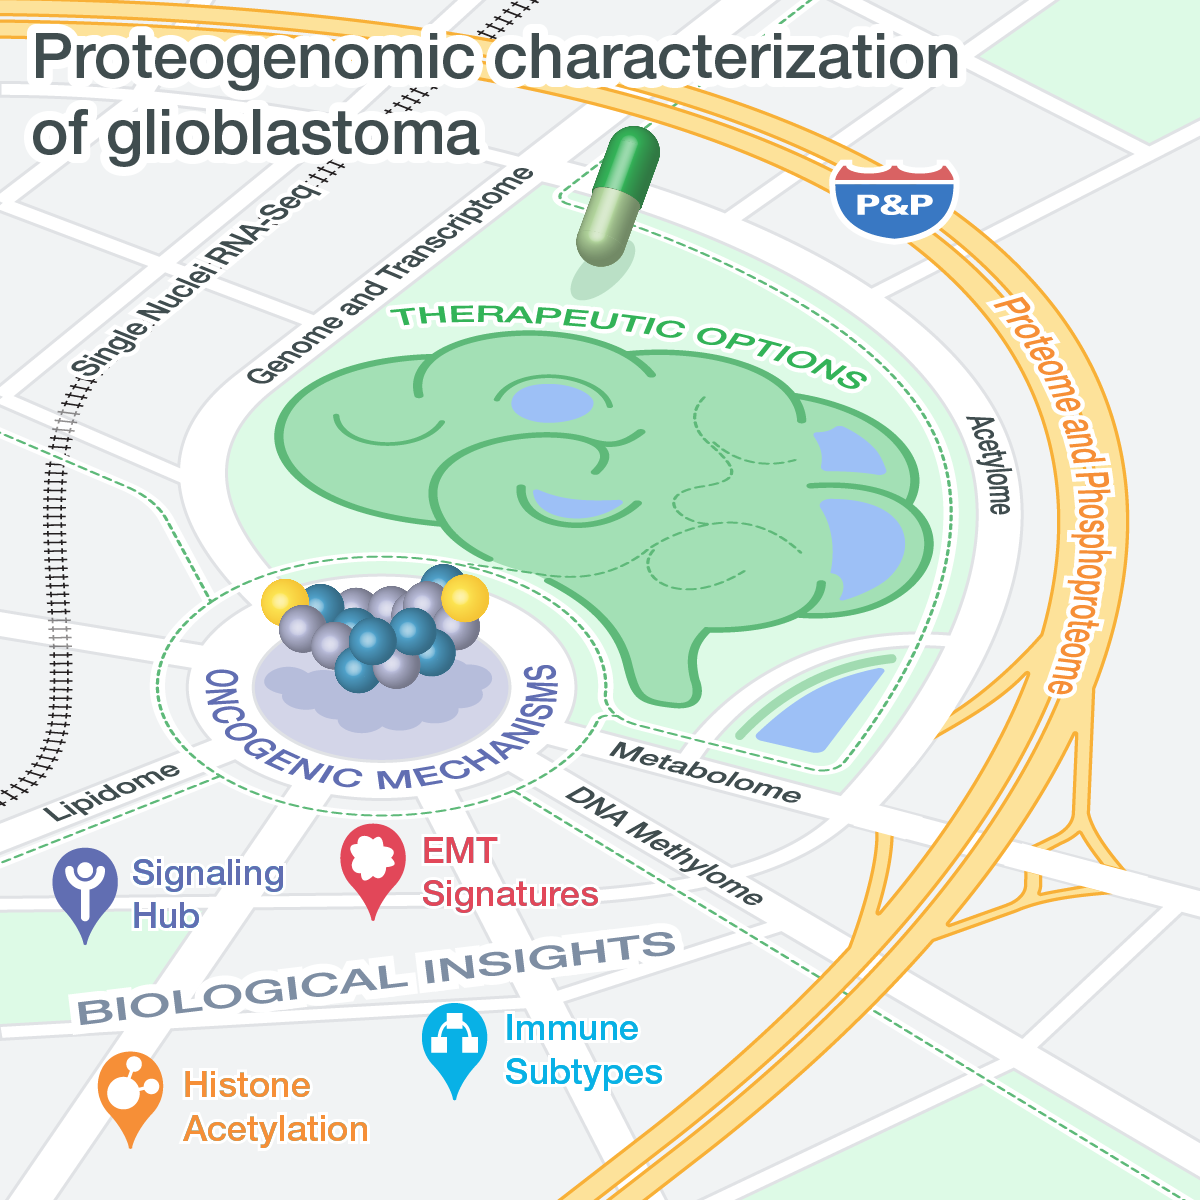
\includegraphics[width=0.5\linewidth]{figures/chap04_cptac_gbm_discov/graphical_abstract.png}
    \caption{Graphical abstract of the CPTAC GBM discovery study.}
    \label{fig:gbm-graphical-abstract}
\end{figure}


\section{Summary}
Glioblastoma (GBM) is the most aggressive nervous system cancer. Understanding its molecular pathogenesis is crucial to improving diagnosis and treatment. Integrated analysis of genomic, proteomic, post-translational modification and metabolomic data on 99 treatment-naive GBMs provides insights to GBM biology. We identify key phosphorylation events (e.g., phosphorylated PTPN11 and PLCG1) as potential switches mediating oncogenic pathway activation, as well as potential targets for \gene{EGFR}-, \gene{TP53}-, and RB1-altered tumors. Immune subtypes with distinct immune cell types are discovered using bulk omics methodologies, validated by snRNA-seq, and correlated with specific expression and histone acetylation patterns. Histone H2B acetylation in classical-like and immune-low GBM is driven largely by BRDs, CREBBP, and EP300. Integrated metabolomic and proteomic data identify specific lipid distributions across subtypes and distinct global metabolic changes in \gene{IDH}-mutated tumors. This work highlights biological relationships that could contribute to stratification of GBM patients for more effective treatment.


\section{Introduction}
Glioblastoma (GBM) is the most common primary malignant brain tumor, with roughly 12,000 new cases annually in the United States and median survival under 2 years \cite{delgado-lopezpd_corrales-garciaem:SurvivalGlioblastoma2016,ostromqt_barnholtz-sloanjs:CBTRUSStatistical2019}. The Cancer Genome Atlas (TCGA) \cite{brennancw_chinl:GBM2013,tcga_network:GBM2008} and other studies \cite{yanh_bignerdd:IDH1IDH22009} have reshaped the World Health Organization classification of nervous system tumors \cite{louisdn_ellisondw:2016World2016} to include molecular features \cite{bratdj_wellerm:CIMPACTNOWUpdate2018, louisdn_vondeimlinga:AnnouncingCIMPACTNOW2017}.
GBM is categorized as either \gene{IDH}-wild type (\gene{IDH}-WT; \textasciitilde90\%) or \gene{IDH}-mutant (\textasciitilde10\%). \gene{IDH}-WT GBMs fall into three distinct subclasses (proneural, classical, and mesenchymal) based on genomic alterations and gene expression signatures \cite{verhaakrgw_hayesdn:IntegratedGenomic2010,wangq_verhaakrgw:TumorEvolution2017}. Methylome-based classification is being used to differentially diagnose brain tumors \cite{karimis_zadehg:CentralNervous2019,nassirif_aldapekd:DNAMethylation2019} and may become clinically useful for GBM.
Surgical resection, chemotherapy, and radiotherapy remain the standard of care \cite{stuppr_mirimanoffro:RadiotherapyConcomitant2005,perryjr_trialinvestigators:ShortCourseRadiation2017}, with the recent addition of tumor treating fields \cite{stuppr_ramz:EffectTumorTreating2017}.
Promising immunotherapies have been proposed, including immune checkpoint inhibitors, vaccines, chimeric antigen receptor T cell (CAR-T) therapy, and viral therapy, though none have cleared Phase III trials \cite{limm_wellerm:CurrentState2018,mcgranahant_nagpals:CurrentState2019}.
Despite different subtypes, no specific treatment works more effectively in a pre-specified subset of patients based on transcriptomics, though those with MGMT promoter methylation respond better to temozolomide \cite{stuppr_mirimanoffro:RadiotherapyConcomitant2005}.

Here, we integrated proteogenomic and metabolomic data from 10 platforms including whole genome sequencing (WGS), whole exome sequencing (WES), RNA sequencing (RNA-seq), microRNA-seq (miRNA-seq), single nuclei RNA-seq (snRNA-seq), DNA methylation arrays, proteome, phosphoproteome, acetylome, lipidome, and metabolome to investigate 99 treatment-naive GBMs prospectively collected by the Clinical Proteomic Tumor Analysis Consortium (CPTAC). We report new immune-based subtypes, activation of DNA repair pathways via upregulated phosphosite levels of DNA repair genes in \gene{TP53}-mutated tumors, an apparent phospho-signaling bottleneck in receptor tyrosine kinase (RTK)-altered tumors, and enrichment of histone H2B acetylation and low macrophage content in classical-like GBM tumors. We used single-cell data to investigate contributions of various cell types to bulk tumor signatures and analyzed the mesenchymal subtype to discern epithelial-mesenchymal transition (EMT) signatures in tumor and infiltrating immune cells. The data presented here furnish a resource for future GBM studies.


\section{Results}

\subsection{Proteogenomic and metabolomic features delineate molecular subtypes of glioblastoma}
We characterized the proteogenomic landscape of 99 GBMs and 10 unmatched GTEx normal brain samples. This cohort has diverse origins and clinical characteristics typical of adult GBM. Six cases harbored \gene{IDH1} R132H mutations and had earlier disease onset than those with \gene{IDH1}-WT (median 47 vs. 59 years, t test p = 0.055). We detected one additional non-hotspot \gene{IDH1} mutation (R222C).

\begin{figure}[p]
    \centering
    \phantomlabel{fig:gbm-overview-data-avail}
    \phantomlabel{fig:gbm-overview-mut-landscape}
    \phantomlabel{fig:gbm-overview-multi-omics}
    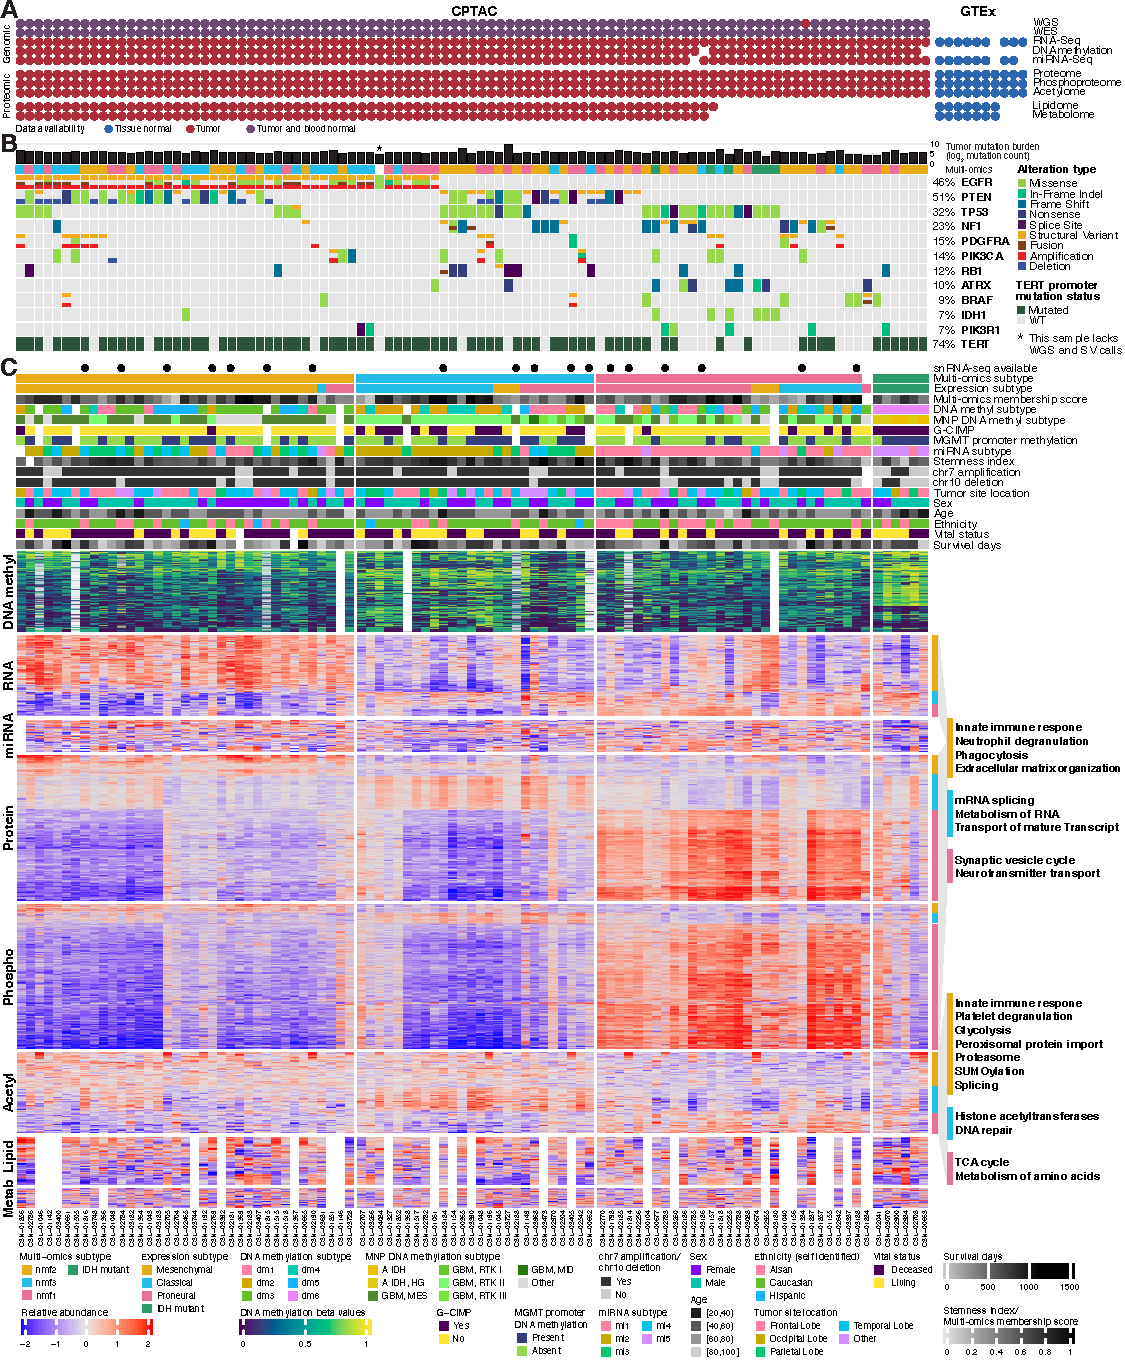
\includegraphics[width=\linewidth]{figures/chap04_cptac_gbm_discov/figure1_overview.pdf}
    \caption[Proteogenomic summary of the cohort.]{%
        Proteogenomic summary of the cohort.
        \legendcontdnote
    }
    \label{fig:gbm-overview}
\end{figure}
\begin{figure}[t]
    \centering
    \legend{%
    \legendcontdref{fig:gbm-overview}
    \subref{fig:gbm-overview-data-avail}
    Summary of 10 data types generated in this study.
    \subref{fig:gbm-overview-mut-landscape}
    Overview of significantly altered genes found in at least 5\% of samples, showing tumor mutation burden ($\log_2$ WES mutation count) and structural variants, fusions, and CNVs. Subtypes are based on results in panel \subref{fig:gbm-overview-multi-omics}.
    \subref{fig:gbm-overview-multi-omics}
    Multi-omics clustering of tumor samples by NMF using CNV, expression, and protein and phosphoprotein abundances. Heatmaps show differential expression between subtypes, including DNA methylation, acetylome, metabolome, and lipidome, and characteristic features for each subtype. Pathway enrichment analysis highlights differences between subtypes. Neuron activity related pathways, immune response pathways, and cell cycle pathways were respectively enriched in the nmf1 (proneural-like), nmf2 (mesenchymal-like), and nmf3 (classical-like) subtypes.
    }
\end{figure}

All samples were homogenized and aliquoted for each of the ten different omics assays (\fref{fig:gbm-overview-data-avail}, \ref{fig:gbm-proteomic-qc-exp-design}--\subcaptionref{fig:gbm-proteomic-qc-corr}). Mass spectrometry (MS) quantified protein, phosphorylation and acetylation, as previously described \cite{douy_zhaog:CPTACUCEC2020,mertinsp_ncicptac:CPTACBreastCancer2016} (\fref{fig:gbm-proteomic-qc-exp-design}--\subcaptionref{fig:gbm-proteomic-qc-corr}). Metabolome and lipidome levels were respectively measured by label-free gas and liquid chromatography coupled to MS. Genomic properties of our cohort were comparable to those of TCGA GBM cohort \cite{brennancw_chinl:GBM2013} (\fref{fig:gbm-overview-mut-landscape}). We identified many structural variants (SV) in oncogenes, including \gene{EGFR} and \gene{PDGFRA}, and tumor suppressors \gene{PTEN} and \gene{NF1}. \gene{EGFR} mutations often co-occurred with \gene{EGFR} SV and amplification events (p < 0.01). WES and WGS identified \gene{TERT} promoter (\gene{TERT}p) mutations with variant allele frequency (VAF) >5\% (\fref{fig:gbm-overview-mut-landscape}). Copy number analysis identified common focal and arm-level copy number variations (CNVs) (\fref{fig:gbm-subtype-gistic}).

\begin{figure}[p]
    \centering
    \phantomlabel{fig:gbm-proteomic-qc-exp-design}
    \phantomlabel{fig:gbm-proteomic-qc-prot-id}
    \phantomlabel{fig:gbm-proteomic-qc-corr}
    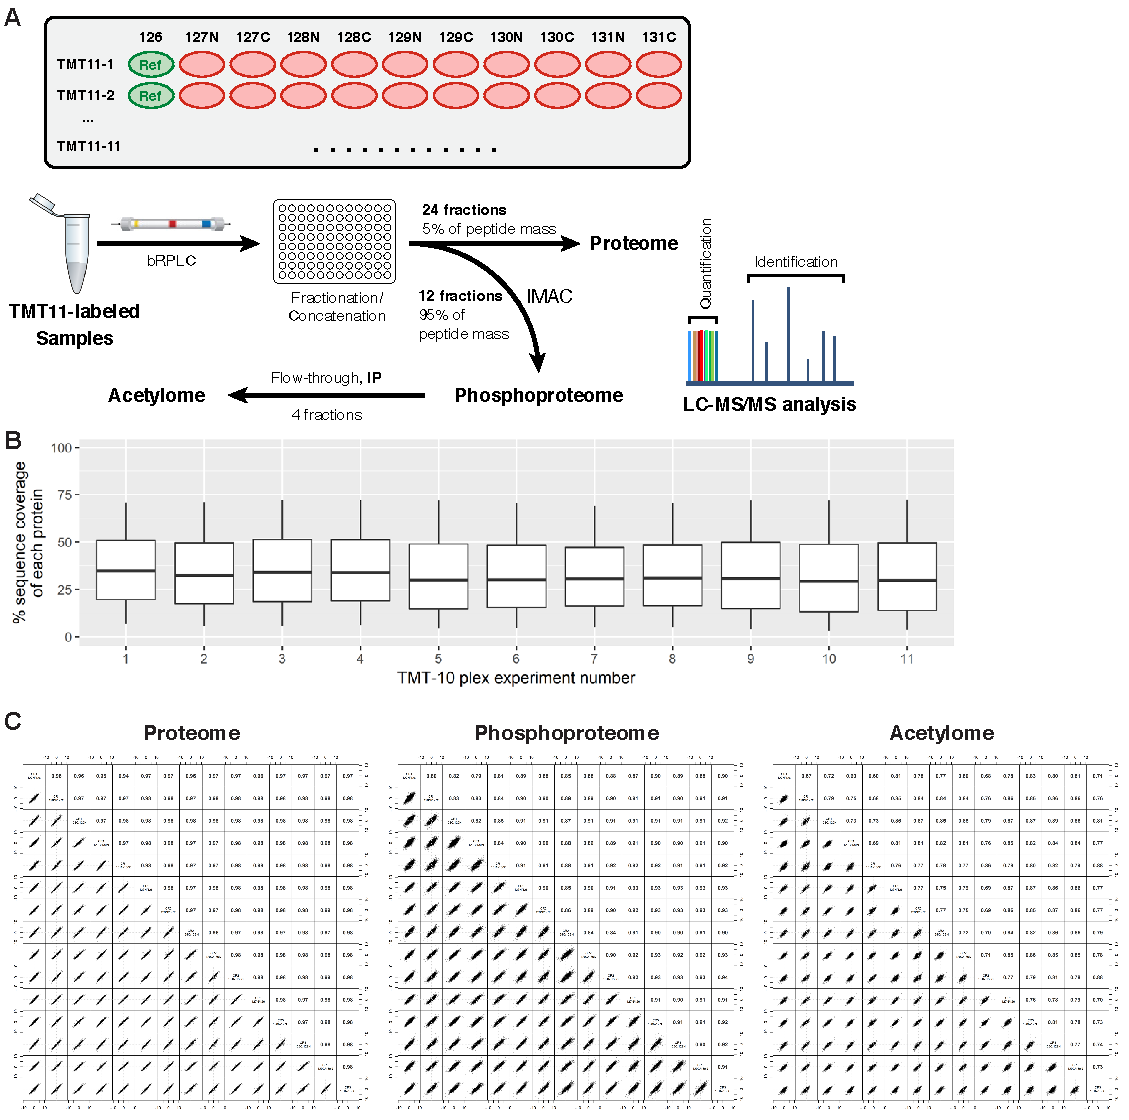
\includegraphics[width=0.9\linewidth]{figures/chap04_cptac_gbm_discov/figures1_proteome_qc.pdf}
    \caption[Integrated proteomic workflow and quality control.]{%
        Integrated proteomic workflow and quality control.
        \subref{fig:gbm-proteomic-qc-exp-design}
        TMT-11 based global proteome, phosphoproteome, and acetylome analysis workflow. The GBM tumors and GTEx normal tissues were analyzed in 11 TMT 11-plex experiments, each with 10 study samples and a common internal reference sample created by pooling all study samples (equal contribution). The TMT11-labeled samples were then fractionated, split (with 5\% peptide mass analyzed directly for global proteome), and subjected to tandem enrichment of phosphopeptides and acetylated peptides. Peptides were detected and quantified using information from the TMT-11 MS/MS spectra.
        \subref{fig:gbm-proteomic-qc-prot-id}
        Distribution of sequence coverage of the identified proteins with tryptic peptides detected by MS/MS in each TMT-11 plex; whiskers show the 5--95 percentiles. The total numbers of identified proteins in each TMT plex range from 9,992 to 10,572.
        \legendcontdnote
    }
    \label{fig:gbm-proteomic-qc}
\end{figure}
\begin{figure}[t]
    \centering
    \legend{%
        \legendcontdref{fig:gbm-proteomic-qc}
        \subref{fig:gbm-proteomic-qc-corr}
        Robust and precise proteomics platforms. Longitudinal performance was tested by repeated proteome, phosphoproteome and acetylome analysis of aliquots of the same patient-derived xenograft QC samples in standalone TMT-11 plexes, along with the GBM study samples; scatter plots and Pearson correlations comparing individual replicate measurements are shown.
    }
\end{figure}

We added protein and phosphosite abundance to prior clustering studies of gene expression (\fref{fig:gbm-overview-multi-omics}, \ref{fig:gbm-subtype}). While our results are concordant with TCGA expression-based classification \cite{wangq_verhaakrgw:TumorEvolution2017}, 27 tumors (29\%) were classified as a different subtype (\fref{fig:gbm-overview-multi-omics}, \ref{fig:gbm-subtype-nmf}).
Based on similarities with gene expression subtypes, we designated the three clusters observed in IDH-WT tumors as nmf1 (proneural-like; n = 29), nmf2 (mesenchymal-like; n = 37), and nmf3 (classical-like; n = 26).
Pathway enrichment analysis of RNA, protein, and phosphosite abundances indicated that nmf1 was enriched for synaptic vesicle cycle and neurotransmission transport; nmf2 was enriched for innate immune response, including neutrophil degranulation, phagocytosis, and extracellular matrix organization; and nmf3 was enriched for mRNA splicing and RNA metabolism.
Based on the known functional effects of protein acetylation \cite{naritat_choudharyc:FunctionsMechanisms2019}, nmf1/proneural-like cluster had a higher abundance of acetylated proteins involved in the TCA cycle and metabolism of amino acids, whereas the nmf2/mesenchymal-like cluster was enriched for innate immune system activation, peroxisomal protein import and glycolysis. The nmf3/classical-like subtype was enriched for acetylation of chromatin modifiers and DNA repair proteins.

\begin{figure}[p]
    \centering
    \phantomlabel{fig:gbm-subtype-gistic}
    \phantomlabel{fig:gbm-subtype-nmf}
    \phantomlabel{fig:gbm-subtype-mixed-subtype}
    \phantomlabel{fig:gbm-subtype-methyl}
    \phantomlabel{fig:gbm-subtype-dnmt}
    \phantomlabel{fig:gbm-subtype-each-data-type}
    \phantomlabel{fig:gbm-subtype-mgmt-survival}
    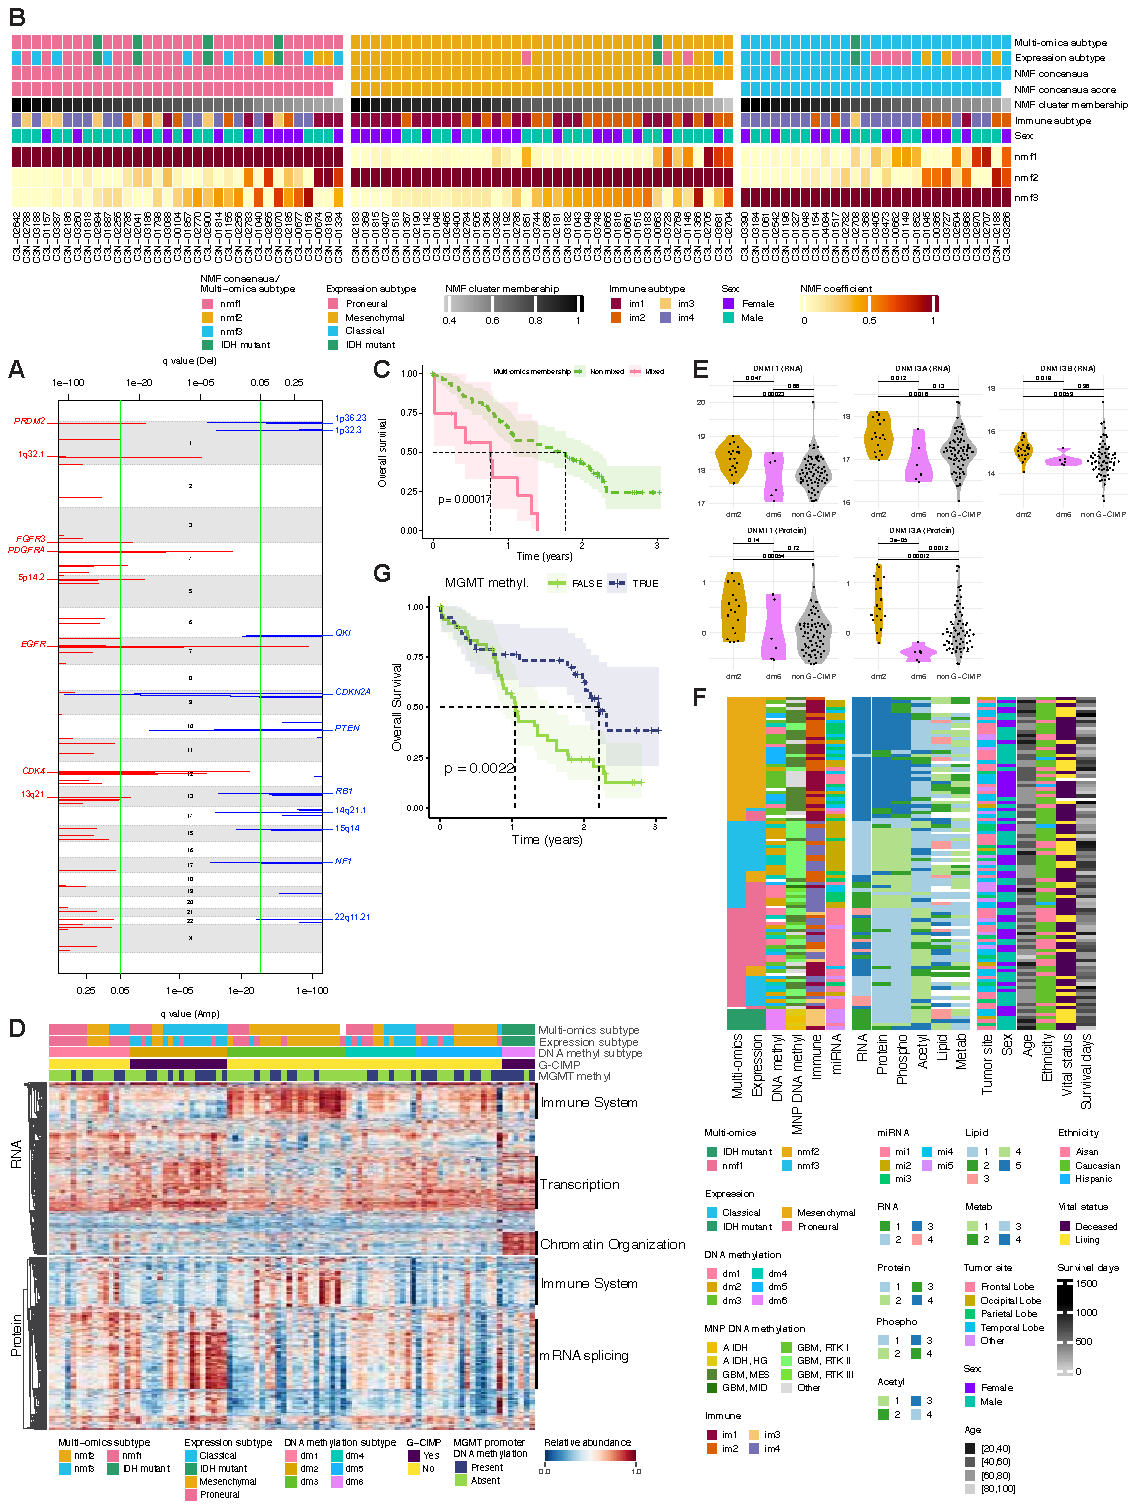
\includegraphics[width=0.95\linewidth]{figures/chap04_cptac_gbm_discov/figures2_subtypes.pdf}
    \caption[Proteogenomic characterization and subtyping of GBM.]{%
        Proteogenomic characterization and subtyping of GBM.
        \legendcontdnote
    }
    \label{fig:gbm-subtype}
\end{figure}
\begin{figure}[t]
    \centering
    \legend{%
        \legendcontdref{fig:gbm-subtype}
        \subref{fig:gbm-subtype-gistic}
        GISTIC2 copy number variations at and focal level of all tumors with WGS available.
        \subref{fig:gbm-subtype-nmf}
        Heatmap of multi-omics membership scores of all three multi-omics subtypes for each tumor.
        \subref{fig:gbm-subtype-mixed-subtype}
        Survival Kaplan–Meier curves of mixed-subtype tumors with low multi-omics membership score versus the rest of the tumors.
        \subref{fig:gbm-subtype-methyl}
        Pathway enrichment analysis of gene expression with differential DNA methylation in promoter regions across all six DNA methylation subtypes.
        \subref{fig:gbm-subtype-dnmt}
        Differentially expressed DNMTs in two G-CIMP subtypes (dm2 and dm6) at both RNA and protein level.
        \subref{fig:gbm-subtype-each-data-type}
        Comparison of the clustering results using individual data type, including DNA methylation, miRNAs, RNAs, proteins, phosphoproteins, acetylproteins, lipids, and metabolites.
        \subref{fig:gbm-subtype-mgmt-survival}
        Survival Kaplan--Meier curves of tumors with different MGMT promoter DNA methylation status.
    }
\end{figure}

Clinical data associated with the three subtypes indicated that tumors with relatively low multi-omics membership scores for two or more subtypes, i.e. those of ``mixed subtype'' (n = 12) (\fref{fig:gbm-subtype-nmf}) were associated with worse prognosis (log rank test p = 1.7e-4; \fref{fig:gbm-subtype-mixed-subtype}) compared with those of non-mixed subtype (excluding \gene{IDH1}-mutant tumors). We identified three proteins associated with poor survival across all tumors: low expression of HIST3H2BB (log rank test p = 0.0034), high expression of MT-CYB (p = 0.03), and high expression of PRODH (p = 0.096).
Genome-wide DNA methylation profiling identified six DNA methylation subtypes, including two distinct glioma CpG island methylator phenotype (G-CIMP) subtypes (dm2 and dm6). The dm6 subtype is IDH-mutant-specific with upregulation of chromatin organization pathways, while dm2 consists of \gene{IDH}-WT tumors with upregulation of transcription and mRNA splicing pathways (\fref{fig:gbm-subtype-methyl}).
Two subtypes showed elevated expression of different \textit{de novo} DNA methylases (\fref{fig:gbm-subtype-dnmt}). We also examined \textit{cis} associations of DNA methylation with RNA or protein abundances using iProFun \cite{songx_wangp:InsightsImpact2019}.
For example, 38 of 90 tumors (42\%) exhibited hypermethylation of the MGMT promoter region and significantly decreased MGMT RNA and protein levels (Welch's t test p = 4.9e-11 and 2.6e-6, respectively) (\fref{fig:gbm-subtype-mgmt-survival}).


\subsection{Driver genetic alterations influence oncogenic protein abundance and phosphorylation}
We associated genetic alterations (mutations, CNVs, fusions, and SVs) with RNA, protein expression and phosphorylation levels, observing 95 \textit{cis-trans} phosphorylation events (\fref{fig:gbm-mut-impact-rna-protein}, \ref{fig:gbm-mut-impact-phospho}). We found strong \textit{cis} effects for \textit{EGFR} and \textit{PDGFRA}, with significant increases in RNA and protein expression and increased phosphorylation at S1166 and S1067/S1070, respectively. At the trans level, tumors with \gene{EGFR} alterations presented elevated CTNNB1 (β-catenin) protein despite decreased mRNA, and increased phosphorylation of both PTPN11 (Shp2) at Y62 and PLCG1 at Y783 (\fref{fig:gbm-mut-impact-rna-protein}, \ref{fig:gbm-mut-impact-phospho}). These observations illustrate the importance of protein measurements to study pathway activation.

\begin{figure}[tb]
    \centering
    \phantomlabel{fig:gbm-mut-impact-rna-protein}
    \phantomlabel{fig:gbm-mut-impact-phospho}
    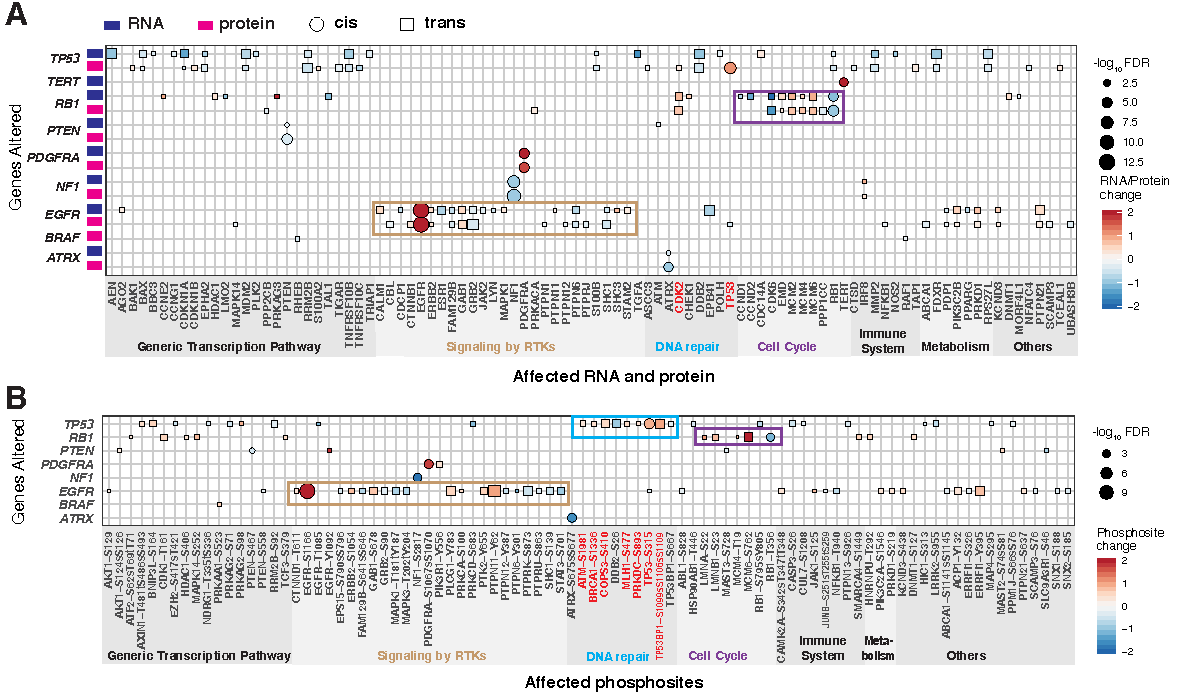
\includegraphics[width=\linewidth]{figures/chap04_cptac_gbm_discov/figure2_mut_impact.pdf}
    \caption[\textit{Cis} and \textit{trans} effects of SMGs on RNA, protein, and phosphorylation abundance.]{%
        \textit{Cis} and \textit{trans} effects of SMGs on protein and phosphorylation.
        \subref{fig:gbm-mut-impact-rna-protein}
        \textit{Cis} and \textit{trans} effects of significantly mutated genes (y axis) on RNA and protein level (x axis) showing that effects are often similar.
        \subref{fig:gbm-mut-impact-phospho}
        \textit{Cis} and \textit{trans} effects of significantly mutated genes (y axis) on protein phosphorylation status (x axis).
    }
    \label{fig:gbm-mut-impact}
\end{figure}

Tumor suppressors \gene{RB1}, \gene{NF1}, \gene{PTEN}, and \gene{ATRX} demonstrated good concordance between genetic alterations and decreased RNA, protein, and phosphorylation levels of their respective gene products. Although the general effect of \gene{TP53} mutations on increased protein stability is known, we identified specific phosphosites that correlate with increased stability. Phosphorylation of TP53 at S315 and TP53BP1 at S1099, S1106, and S1109 correlated with increased TP53 protein expression (Pearson r = 0.89 and 0.53, respectively) (\fref{fig:gbm-mut-impact-rna-protein}, \ref{fig:gbm-mut-impact-phospho}).

We assessed kinases known to phosphorylate TP53 and its downstream targets. In TP53 mutants (\fref{fig:gbm-mut-impact-rna-protein}, \ref{fig:gbm-mut-impact-phospho}), we detected elevated protein and/or phosphorylation in ATR, MAPK3, CDK2, and CDK9, while MDM2 was decreased at both RNA and protein levels. Tumors with \gene{TP53} mutations showed upregulated phosphosites, but not increased protein levels, of DNA repair genes, suggesting specific phosphosite regulation. We observed negative feedback between RB1 and downstream targets, CDK2, CDK6, MCM2, MCM4, and MCM6, while NF1 had similar effects on IRF8 (\fref{fig:gbm-mut-impact-rna-protein}, \ref{fig:gbm-mut-impact-phospho}). \gene{RB1}-altered samples (12\% of the cohort) showed significantly downregulated RB1 and upregulated MCM2, MCM4, and MCM6 protein expression. In addition, in samples with \gene{NF1} alterations, we observed upregulation of protein and RNA of IRF8, a transcription factor that controls microglial motility \cite{masudat_inouek:IRF8Transcriptional2014} (\fref{fig:gbm-mut-impact-rna-protein}, \ref{fig:gbm-mut-impact-phospho}).


\subsection{RTK signaling cascades are activated in GBM}
% TODO: simplify me
Genomic loci associated with RTKs, such as EGFR, PDGFRA, and MET, are frequently amplified in GBM \cite{brennancw_chinl:GBM2013}. We identified 45 tumors with \gene{EGFR} SVs, all having copy number amplifications, suggesting high concordance between SV and CNV (\fref{fig:gbm-overview-mut-landscape}). All tumors with mutated \gene{EGFR} and SV have correspondingly high RNA, protein, and Y1172 phosphorylation levels, indicating EGFR pathway activation. We did not find expression differences between samples having a sole SV event versus those with dual mutation and SV events, suggesting EGFR upregulation in GBM is largely due to SV, as associated with CNV amplification, rather than mutationally driven, which is different from other tumor types, such as lung cancer \cite{tcga:LUAD2014}. We also found nine samples in which \gene{EGFR} SV co-occurred with \gene{PDGFRA} or \gene{FGFR3} SV, while 13 samples with either \gene{PDGFRA} or \gene{FGFR3} alteration did not show any alterations in \gene{EGFR}. For \gene{PDGFRA}, two out of three mutations overlap with SV events. Only one sample with mutation in \gene{PDGFRA} had high PDGFRA RNA and protein expression. For EGFR, n = 53 (WT), 29 (SV), and 16 (SV and MUT); for \gene{PDGFRA}, n = 84 (WT), 12 (SV), and 2 (SV and MUT).

\begin{figure}[tb]
    \centering
    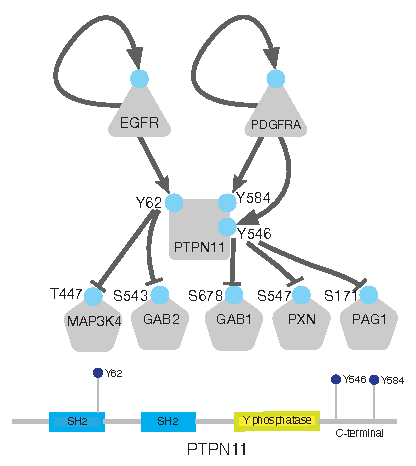
\includegraphics[width=0.5\linewidth]{figures/chap04_cptac_gbm_discov/figure3_ptpn11.pdf}
    \caption[Alterations in RTKs and associations with expression, phosphosite status, and downstream targets.]{%
        Alterations in RTKs and associations with expression, phosphosite status, and downstream targets. The schematic shows dual regulation of PTPN11 by EGFR and PDGFRA and the downstream substrates that PTPN11 may dephosphorylate.
    }
    \label{fig:gbm-ptpn11}
\end{figure}

We also observed increased phosphorylation levels of PTPN11-Y62, PLCG1-Y783, RB1-S795Y805, MAP3K1-S1408, and specific EGFR sites in \gene{EGFR}-altered samples. Notably, the total protein level of PTPN11 was comparable between the two groups, suggesting its activity is regulated primarily by phosphorylation. A similar pattern is observed with PLCG1 (PLCγ1), where Y783 phosphorylation was significantly higher in \gene{EGFR}-altered versus \gene{EGFR}-WT samples (Wilcox false discovery rate [FDR] < 0.01; \fref{fig:gbm-rtk-ihc-plcg1-gab}), despite no significant difference in PLCγ1 protein expression (FDR = 0.11). Since phosphorylation of PLCG1 on Y783 is activating \cite{poulinb_rheesg:IntramolecularInteraction2005}, this could provide a mechanism for EGFR activation of PLCG1’s known effects on proliferation, migration, and invasiveness \cite{kunzek_brauningera:RecurrentActivating2014}.

\begin{figure}[p]
    \centering
    \phantomlabel{fig:gbm-rtk-ihc-alter-impact}
    \phantomlabel{fig:gbm-rtk-ihc-fgfr3-fusion}
    \phantomlabel{fig:gbm-rtk-ihc-plcg1-gab}
    \phantomlabel{fig:gbm-rtk-ihc-ihc-sox9-gab1}
    \phantomlabel{fig:gbm-rtk-ihc-ihc-im1-im4}
    \phantomlabel{fig:gbm-rtk-ihc-ihc-all-ims}
    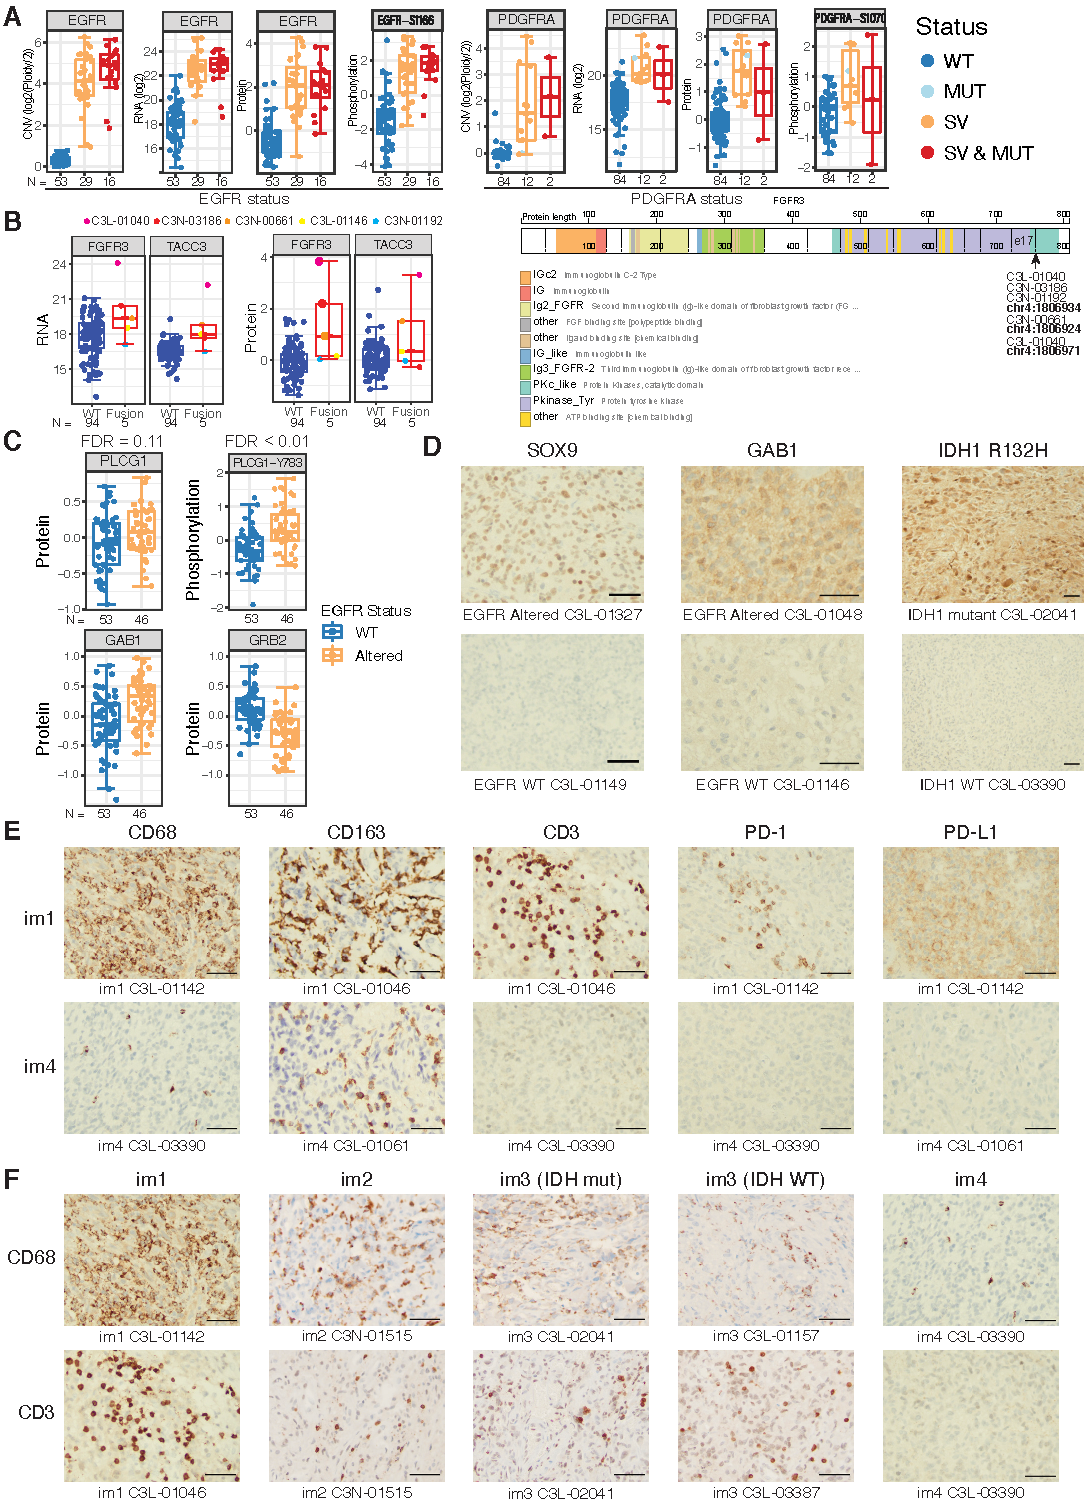
\includegraphics[height=0.93\textheight]{figures/chap04_cptac_gbm_discov/figures4_validation.pdf}
    \caption[RNA, protein and phosphosite level change in samples with different RTK alterations, and IHC validations.]{%
        RNA, protein and phosphosite level change in samples with different RTK alterations, and IHC validations.
        \legendcontdnote
    }
    \label{fig:gbm-rtk-ihc}
\end{figure}
\begin{figure}[t]
    \centering
    \legend{%
        \legendcontdref{fig:gbm-rtk-ihc}
        \subref{fig:gbm-rtk-ihc-alter-impact}
        The comparison of CNV, RNA and protein expressions and phosphosite level between EGFR altered and WT samples (left panel) and PDGFRA altered and WT samples (right panel).
        \subref{fig:gbm-rtk-ihc-fgfr3-fusion}
        The comparison of RNA and protein expression of FGFR3 and TACC3 between samples with and without FGFR3-TACC3 fusion and the breakpoints found in FGFR3 from RNA-Seq data (n = 94 and 5, respectively). Five samples with FGFR3-TACC3 fusions with an intact FGFR3 kinase domain. Three samples which are protein expression outliers in FGFR3 are marked by larger circles.
        \subref{fig:gbm-rtk-ihc-plcg1-gab}
        The comparison of PLCG1, GAB1, and GRB2 protein expression and PLCG1-Y783 phosphosite level between EGFR altered (n = 46) and WT (n = 53) samples.
        \subref{fig:gbm-rtk-ihc-ihc-sox9-gab1}
        Immunohistochemistry staining for SOX9 and GAB1 expression in EGFR altered and WT tumors is concordant with the mass spectrometry findings. Positive IDH1 R132H staining of the ATRX WT and IDH1 mutant tumor. Scale bars: 100 μm.
        \subref{fig:gbm-rtk-ihc-ihc-im1-im4}
        Immunohistochemistry staining for CD68, CD163, CD3, PD-1, PD-L1 in tumors of different immune subtypes is concordant with the mass spectrometry and gene expression analyses. Scale bars: 100 μm.
        \subref{fig:gbm-rtk-ihc-ihc-all-ims}
        Immunohistochemistry staining for CD68 and CD3 in tumors of all four immune subtypes is concordant with the mass spectrometry and gene expression analyses. Scale bars: 100 μm.
    }
\end{figure}

We performed a kinase-substrate study for EGFR and PDGFRA and identified high levels of GAB1 phosphorylation at Y689 and Y657, consistent with high EGFR expression. In addition, PTPN11 phosphosites at Y546 and Y584 were associated with high PDGFRA expression (\fref{fig:gbm-ptpn11}) and have been observed in lung cancers with ALK fusions \cite{voenac_chiarler:TyrosinePhosphatase2007}. Activation of PTPN11 through either EGFR- or PDGFRA-related phosphorylation in GBM suggests it may represent a shared RTK signaling hub. PTPN11, GAB1, and GRB2 form a complex and are co-regulated by RTKs to activate the RAS pathway \cite{montagnera_raynalp:NovelRole2005}. Figures \ref{fig:gbm-mut-impact-rna-protein} and \ref{fig:gbm-rtk-ihc-plcg1-gab} show that EGFR activation status is associated with upregulated GAB1 and downregulated GRB2 protein expression. We validated the elevated GAB1 expression in EGFR-altered tumors using IHC (\fref{fig:gbm-rtk-ihc-ihc-sox9-gab1}).


\subsection{Distinct immune marker expression and epigenetic events characterize GBM immune subtypes}
We generated cell-type immune enrichment scores using single-sample GSEA by xCell \cite{arand_butteaj:XCellDigitally2017}, finding four distinct immune-based GBM subtypes (\fref{fig:gbm-immune-deconv}). Immune subtype 1 (im1) showed overall higher scores (\fref{fig:gbm-immune-valid-tcga-score}), including elevated levels of microglia, macrophages, and lymphocytes. Immune subtypes 2 and 3 (im2 and im3) displayed reciprocal ratios of macrophages and lymphocytes, with im2 higher in macrophages and lower in lymphocytes and im3 having higher neuron score (\fref{fig:gbm-immune-deconv} and \ref{fig:gbm-immune-valid-tcga-score}). Immune subtype 4 (im4) is distinct from the others, with substantially lower enrichment for all immune cell types (\fref{fig:gbm-immune-deconv} and \ref{fig:gbm-immune-valid-tcga-score}). The mesenchymal subtype was enriched in im1 and im2 (Fisher test p = 1.65e-15), while IDH mutants were overrepresented in im3 (p = 1.02e-5). The DNA methylation dm3 subtype was strongly associated with im1 (Fisher test p = 1.26e-5), consistent with the association of dm3 with immune gene expression (\fref{fig:gbm-subtype-methyl}). The four immune subtypes were confirmed in the TCGA GBM cohort using transcriptome data (\fref{fig:gbm-immune-valid-tcga-score} and \ref{fig:gbm-immune-valid-tcga-cluster}) and protein deconvolution (\fref{fig:gbm-immune-deconv} and \ref{fig:gbm-immune-valid-protein-cibersort}).

\begin{figure}[p]
    \centering
    \phantomlabel{fig:gbm-immune-deconv}
    \phantomlabel{fig:gbm-immune-histo-umap}
    \phantomlabel{fig:gbm-immune-histo-example-im4}
    \phantomlabel{fig:gbm-immune-histo-example-not-im4}
    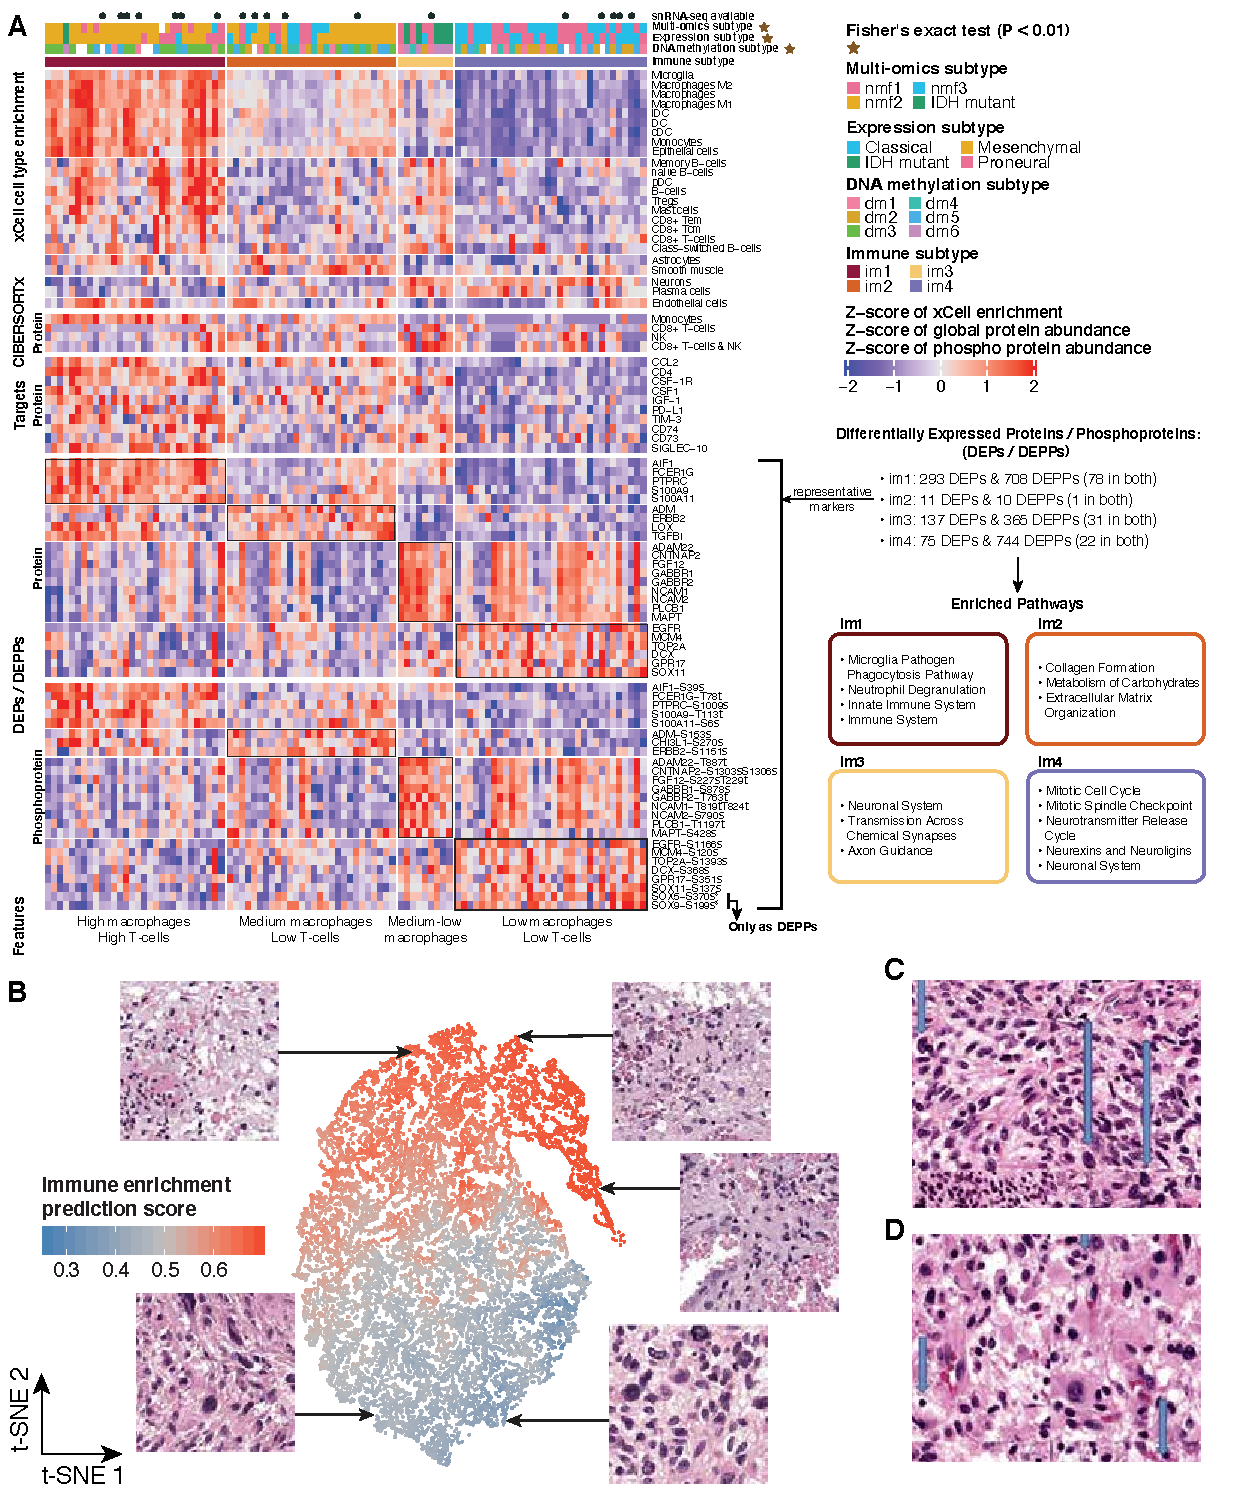
\includegraphics[width=\linewidth]{figures/chap04_cptac_gbm_discov/figure4_immune.pdf}
    \caption[Cell-type enrichment, immune marker expression, and enrichment pathways among the four immune subtypes.]{%
        Cell-type enrichment, immune marker expression, and enrichment pathways among the four immune subtypes.
        \legendcontdnote
    }
    \label{fig:gbm-immune}
\end{figure}
\begin{figure}[t]
    \centering
    \legend{%
        \legendcontdref{fig:gbm-immune}
        \subref{fig:gbm-immune-deconv}
        The four immune subtypes identified by consensus clustering showing cell-type features, immune checkpoints, and potential immunotherapy targets. Differential expression is between tumors of one immune subtype versus the rest based on global protein and phosphoprotein abundance (DEPs/DEPPs: FDR <0.05 and log\textsubscript{2}FC > 0.8) and the corresponding enriched pathways (FDR <0.05 and log\textsubscript{2}FC ≥ 3 markers included in the pathway).
        \subref{fig:gbm-immune-histo-umap}
        Features captured by the deep learning model. Each dot represents a tile of H\&E slides in the test set, colored according to prediction score (red: predicted immune-high; blue: predicted immune-low). The 20,000 sampled tiles from 99 patients were clustered by t-SNE to their activation maps (a 1,250-long vector for each tile) from the final layer of the model.
        \subref{fig:gbm-immune-histo-example-im4}
        H\&E tile images from im4 tumors, with arrows indicating giant cells. The highlighted region contains multiple noncontinuous tiles clustered closely in t-SNE space.
        \subref{fig:gbm-immune-histo-example-not-im4}
        H\&E tile images from non-im4 tumors, with arrows indicating the inflammatory cells. The highlighted region contains multiple noncontinuous tiles clustered closely in t-SNE space.
    }
\end{figure}

We performed snRNA-seq on 18 GBM samples using the same cryopulverized material from previous analyses (7 im1, 5 im2, 1 im3, 5 im4 samples; \fref{fig:gbm-immune-deconv}). TAMs comprised the major non-neoplastic cell population in the GBM TME (\fref{fig:gbm-single-cell-umap}). Im4 samples showed consistently low percentages of T cell and TAM infiltration (1.3\% and 6\% on average, respectively) compared with those of the other immune subtypes (7\% and 19\% on average, respectively). Im1 tumors showed higher scores for microglia and macrophages at the bulk level, but this was not observed in im1--3 in snRNA-seq (\fref{fig:gbm-immune-valid-sc-percentage}), which may be explained by the bulk data being driven by the percentage of TAMs and the expression of genes in the TAMs themselves. We validated key immune markers (CD3, CD68, CD163, PD-1, and PD-L1) in five tumors from three immune subtypes using IHC (\fref{fig:gbm-rtk-ihc-ihc-im1-im4} and \ref{fig:gbm-rtk-ihc-ihc-all-ims}).

\begin{figure}[tb]
    \centering
    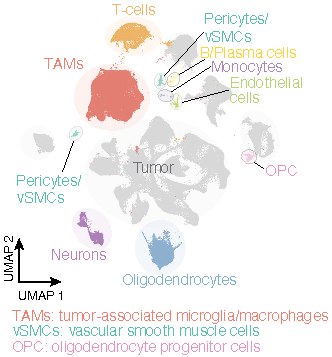
\includegraphics[width=0.5\linewidth]{figures/chap04_cptac_gbm_discov/figure4_immune_single_cell.pdf}
    \caption[Overview of the snRNA-seq cell type annotation.]{%
        snRNA-seq UMAP plot colored by cell types observed in 18 discovery cohort GBM samples. OPC, oligodendrocyte progenitor cells; TAM, tumor-associated microglia/macrophage; vSMC, vascular smooth muscle cell.
    }
    \label{fig:gbm-single-cell-umap}
\end{figure}

We identified differentially expressed proteins (DEPs) and phosphoproteins (DEPPs) in known immune targets \cite{chenz_hambardzumyand:ImmuneMicroenvironment2018}. Gene and protein expression levels of immune targets, including negative regulatory immune checkpoints (e.g., PD-1 and TIM-3), chemokines (e.g., CCL2), macrophage-specific cytokines (e.g., CSF-1), and their receptors (CSF-1R), were significantly higher in im1 (\fref{fig:gbm-immune-deconv}) \cite{butowskin_pradosm:OrallyAdministered2016}. We also identified overrepresented pathways among DEPs and DEPPs. Pathways in im1, including immune system and microglia pathogen phagocytosis, were mostly immune-related, whereas collagen formation and angiogenesis-related proteins were upregulated in im2, neuronal system pathways in im3, and cell cycle and gliogenesis pathways in im4 (\fref{fig:gbm-immune-deconv}).

We analyzed morphologic differences between immune subtypes by applying a deep learning model using sampled tumor tiles from H\&E-stained sections. Dimensional reduction (t-SNE) of im4 compared with other clusters (im1--3) (\fref{fig:gbm-immune-histo-umap}, \ref{fig:gbm-immune-histo-example-im4}, \ref{fig:gbm-immune-histo-example-not-im4}) revealed a substantial number of large cells, some of which are giant cells, in im4 tiles, with few in im1--3 tiles. Biological relevance of these cells is unclear. Inflammatory cell fractions were noted in \textasciitilde20\% of im1--3 tiles compared to 5\% in im4 tiles.

\begin{figure}[tbp]
    \centering
    \phantomlabel{fig:gbm-immune-valid-tcga-score}
    \phantomlabel{fig:gbm-immune-valid-tcga-cluster}
    \phantomlabel{fig:gbm-immune-valid-protein-cibersort}
    \phantomlabel{fig:gbm-immune-valid-sc-percentage}
    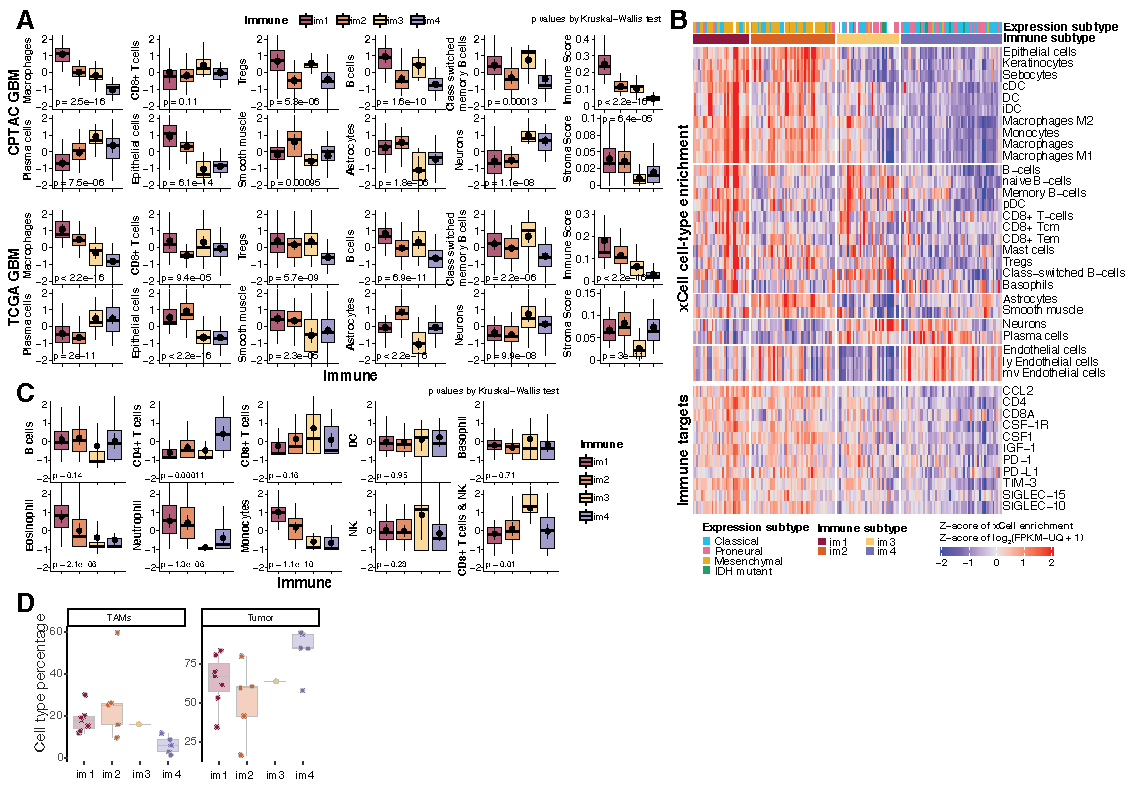
\includegraphics[width=\linewidth]{figures/chap04_cptac_gbm_discov/figures5_immune.pdf}
    \caption[Distinct Immune Marker Expression Ascertains Immune Subtypes.]{%
        Distinct Immune Marker Expression Ascertains Immune Subtypes.
        \subref{fig:gbm-immune-valid-tcga-score}
        The distributions of xCell cell type enrichments, immune scores, and stroma scores among the 4 immune subtypes in the CPTAC GBM cohort and TCGA GBM cohort. For CPTAC, n = 30 (im1), 28 (im2), 9 (im3), and 32 (im4); for TCGA, n = 32 (im1), 48 (im2), 35 (im3), and 59 (im4).
        \subref{fig:gbm-immune-valid-tcga-cluster}
        The 4 immune subtypes identified by the consensus clustering on the cell type enrichment in the TCGA GBM study.
        \subref{fig:gbm-immune-valid-protein-cibersort}
        The distributions of protein-based CIBERSORT cell type enrichments among the 4 immune sub- types in the CPTAC GBM cohort. n = 30 (im1), 28 (im2), 9 (im3), and 32 (im4).
        \subref{fig:gbm-immune-valid-sc-percentage}
        snRNA-seq cell type percentage per sample in each immune subtypes.
    }
    \label{fig:gbm-immune-valid}
\end{figure}


\subsection{Mesenchymal tumor and microenvironment characteristics}
Application of CausalPath \cite{baburo_demire:CausalInteractions2018} to the protein and phosphoprotein expression data (\fref{fig:gbm-pathway-supp-mes}) showed upregulation of the hypoxia pathway in mesenchymal tumors, evidenced by significant activation of multiple HIF-1 downstream targets (network permutation p = 0.0012). Increased angiogenesis was also evident in mesenchymal tumors, as demonstrated by upregulation of FLT1, MMP14, ENG, and SERPINE1. We observed complex regulation of macrophage activation and polarization through the upregulation of STAT3, ICAM1, SPI1, and CEBPB. In addition, the M1 polarization marker ARG1 showed increased expression \cite{arlauckassp_weisslederr:Arg1Expression2018}, along with SERPINE1 and HCK proteins, which promote M2 polarization \cite{kubalamh_declerckya:PlasminogenActivator2018}. The elevated inflammatory response in mesenchymal tumors may result in downstream activation of either hypoxia or macrophage polarization through multiple mediators, including LANE, IL18, and CD40 (\fref{fig:gbm-pathway-supp-mes}).


\subsection{Differential acetylation of histone proteins is associated with specific subtypes and pathways}
Histone acetylation regulates gene expression but is frequently aberrant in cancer \cite{eberhartera_beckerpb:HistoneAcetylation2002}. We detected more than 30 acetylation sites on histones H1, H2A, H2B, H3.3, and H4. Unsupervised clustering of these sites across all samples identified subsets of tumors with differentially acetylated histones H1, H2B, H3.3, and H4 (\fref{fig:gbm-histone-acetyl}). Histone acetylation was generally upregulated in tumors compared to normal samples, with a subset of tumors having elevated H1, H3, and H4 acetylation, while a different cluster exhibited significantly increased acetylation of H2B N-terminal sites (\fref{fig:gbm-histone-acetyl}).

\begin{figure}[tb]
    \centering
    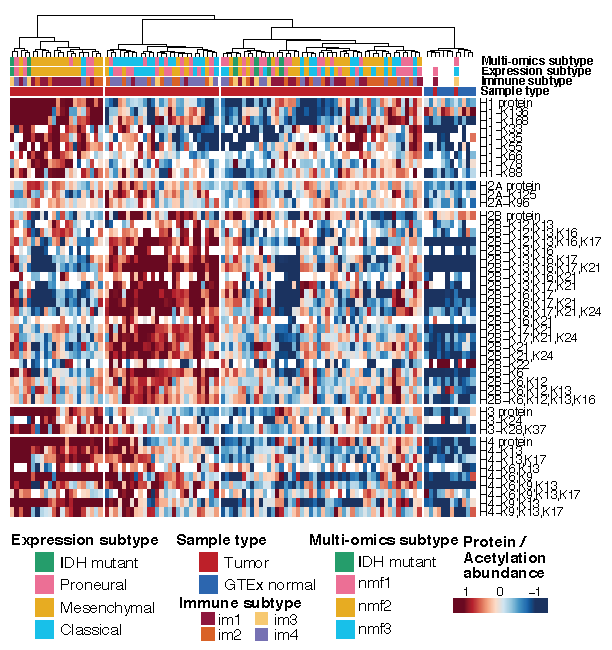
\includegraphics[width=0.6\linewidth]{figures/chap04_cptac_gbm_discov/figure5_histone_acetyl.pdf}
    \caption[Histone acetylation associations with immune subtypes and pathways.]{%
        Histone acetylation associations with immune subtypes and pathways.
        Unsupervised clustering of histone protein and site-level acetylation reveals distinct clusters of tumors enriched for acetylation of histones H2B, H3, and H4.
    }
    \label{fig:gbm-histone-acetyl}
\end{figure}


\subsection{Key oncogenic pathways and therapeutic opportunities in GBM}
We integrated genetic alterations and the RNA, protein, and phosphosite levels per expression subtype to examine three important oncogenic signaling pathways in GBM: RTK/RAS, PI3K/AKT, and p53/cell cycle (\fref{fig:gbm-pathway-summary}). We found that expression outlier percentage was much higher than genetic alteration rate in RTK pathways. Moreover, analyzed tumors harbored at least one genetic alteration or outlier expression in at least one of the three pathways.

\begin{figure}[tb]
    \centering
    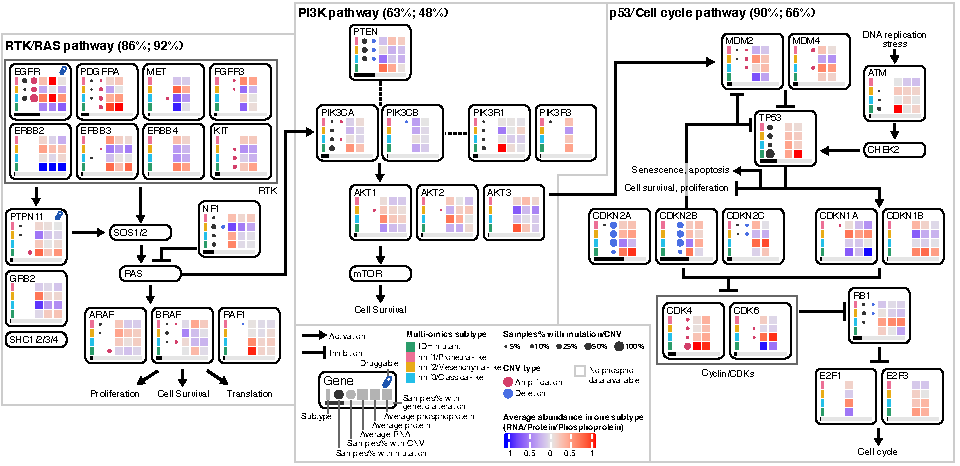
\includegraphics[width=\linewidth]{figures/chap04_cptac_gbm_discov/figure7a_pathway_summary.pdf}
    \caption[Summary of pathway alterations.]{%
        Three oncogenic pathways frequently altered in GBM. Each gene is annotated with mutational and CNV frequency, RNA, protein, and phosphoprotein abundance, by multi-omics subtype. Horizontal bar below gene box indicates frequency of alteration across all tumors. Also indicated are the proportion of tumors with genetic alterations (first percentage) and protein and phosphoprotein outlier expression (second percentage) for each pathway.
    }
    \label{fig:gbm-pathway-summary}
\end{figure}

In the RTK/RAS pathway, classical tumors predominantly showed amplified \gene{EGFR}, while proneural and \gene{IDH}-mutant tumors showed amplified \gene{PDGFRA}, both resulting in higher RNA, protein, and phosphosite abundances of EGFR and PDGFRA, respectively, illustrating convergence at the functional level. For mesenchymal tumors, we observed upregulated MET and downregulated NF1 protein abundance.

In the PI3K pathway, proneural, mesenchymal, and classical tumors showed lower expression of PTEN due to mutations and deletions, which potentially activate AKT1 and AKT2 through phosphatidylinositol (3,4,5)-trisphosphate (PIP\textsubscript{3}). In contrast, AKT3 expression was higher in IDH-mutant and proneural tumors, explained by active expression of \gene{AKT3} in adult brains \cite{eastonrm_birnbaummj:RoleAkt32005}. In the p53/cell cycle pathway, we observed subtype-specific amplification and increased expression of \gene{MDM2} in mesenchymal and MDM4 in proneural and classical tumors. We also observed differences between \gene{IDH} WT and mutant tumors in \gene{CDKN2A/B}.

\begin{figure}[tb]
    \centering
    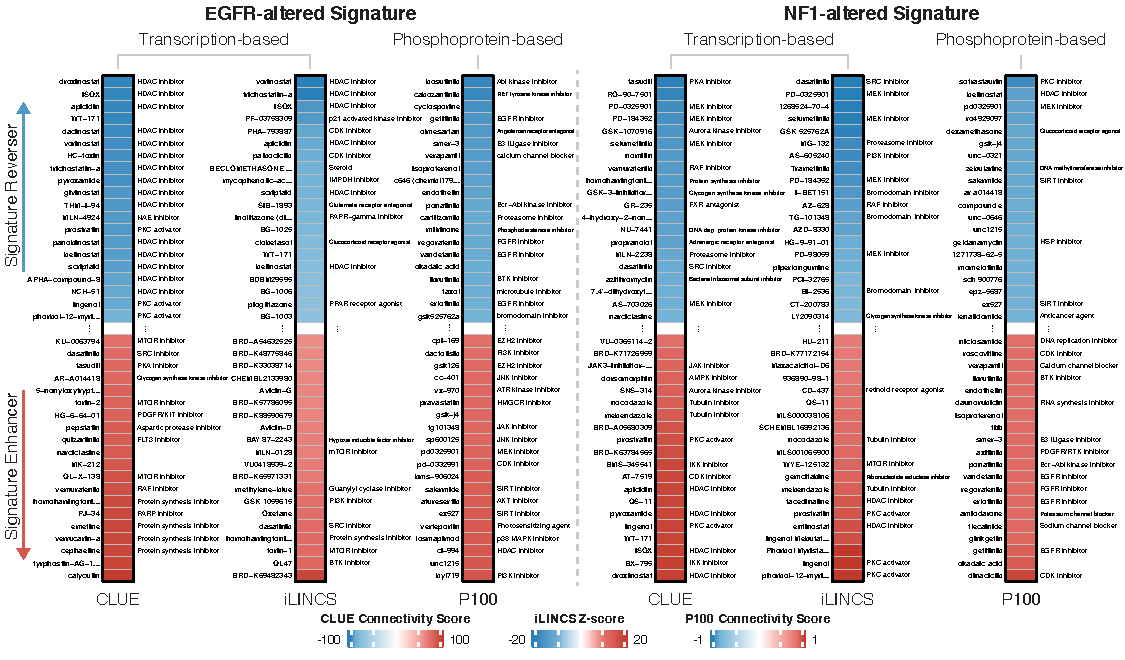
\includegraphics[width=\linewidth]{figures/chap04_cptac_gbm_discov/figure7c_drug_connectivity_signature.pdf}
    \caption[Summary of potential therapeutic targets.]{%
        Summary of potential therapeutic targets. Drug connectivity analysis using alteration-specific transcriptional (CLUE and iLINCS) and phosphoproteomic (P100) signatures (altered tumors versus WT tumors). Twenty compounds that most strongly reverse or enhance the signature are highlighted along with their known mechanisms of action.
    }
    \label{fig:gbm-druggability}
\end{figure}

Using the Library of Integrated Network-Based Cellular Signatures (LINCS) \cite{keenanab_pillaia:LibraryIntegrated2018,stathiasv_schurersc:LINCSData2019}, we calculated the similarity between alteration-specific RNA or phosphoprotein signatures from our study with corresponding transcriptional (L1000 assay) \cite{subramaniana_golubtr:NextGeneration2017} and phosphoproteomic LINCS signatures (P100 assay) \cite{litichevskiyl_jaffejd:LibraryPhosphoproteomic2018} to identify compounds predicted to reverse tumor signatures of the cohort. Phosphoproteomic data yielded more robust results than the transcriptional-response data. For example, while RNA signatures suggested that HDAC inhibitors might reverse the EGFR signature, phosphoproteomic data indicated kinase inhibitors, beyond the expected EGFR inhibitors, to be more highly connected with potential inhibitory effects (\fref{fig:gbm-druggability}). In contrast, NF1-altered samples exhibited concordance between the transcriptional and phosphoproteomic perturbation-response analyses: both suggested MAPK inhibitors as top signature-reversing candidates (\fref{fig:gbm-druggability}). RB1 alteration and immune subtypes agreed variously when comparing perturbations predicted to reverse the gene-altered cell states using transcriptomics versus phosphoproteomics readouts \fref{fig:gbm-pathway-supp-rb1-druggability}).

\begin{figure}[p]
    \centering
    \phantomlabel{fig:gbm-pathway-supp-mes}
    \phantomlabel{fig:gbm-pathway-supp-rb1-druggability}
    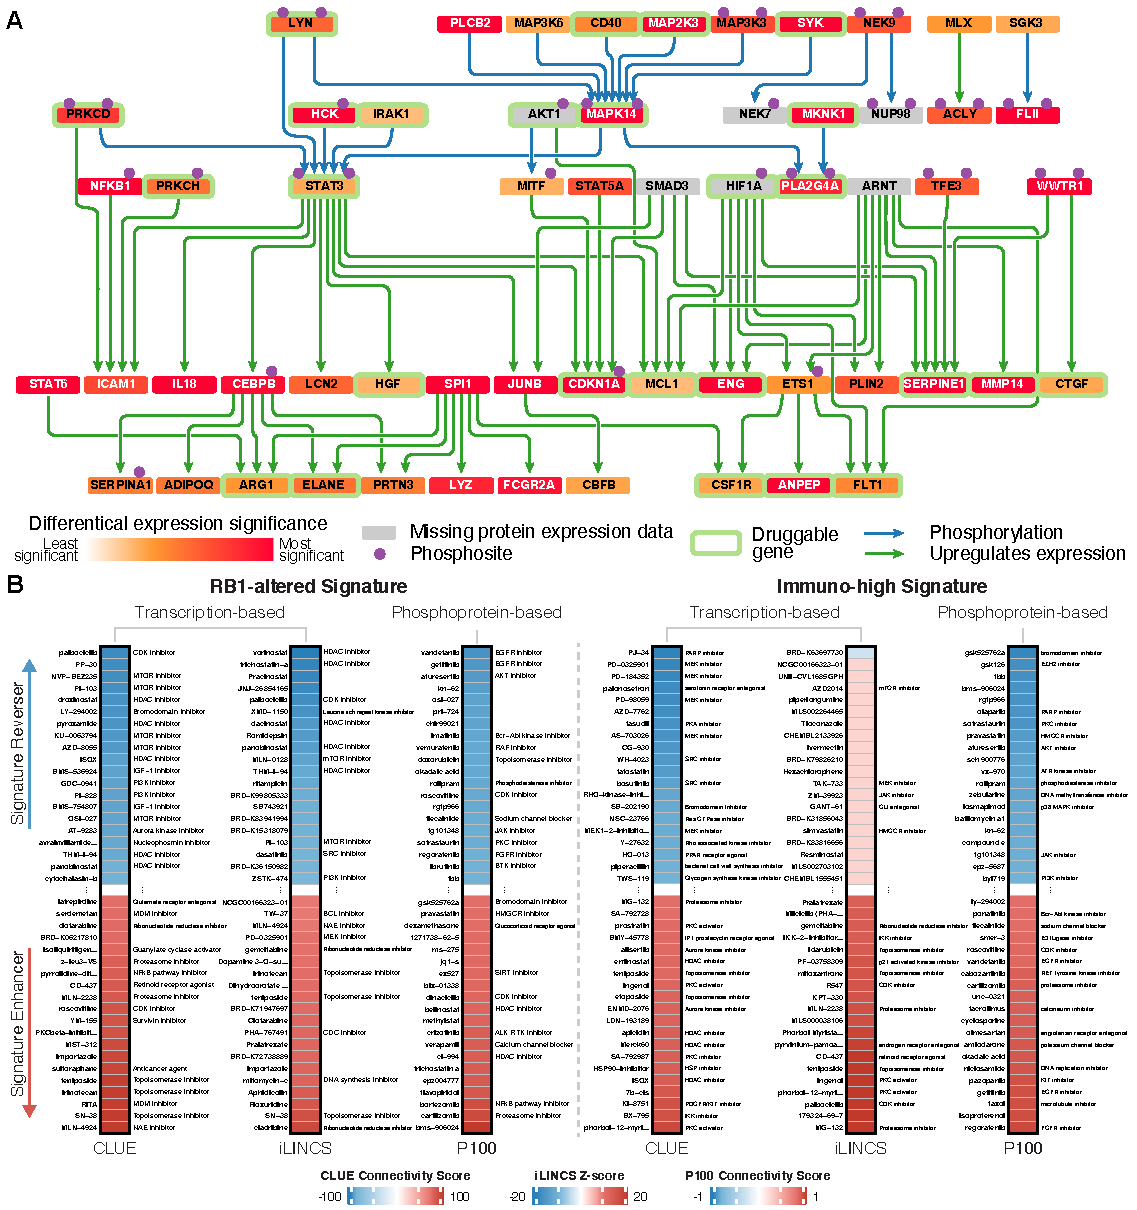
\includegraphics[width=\linewidth]{figures/chap04_cptac_gbm_discov/figures7_pathway_druggability.pdf}
    \caption[Summary of Pathway Alterations of Mesenchymal Tumors Compared to the Other Tumors.]{%
    Summary of Pathway Alterations of Mesenchymal Tumors Compared to the Other Tumors.
        \legendcontdnote
    }
    \label{fig:gbm-pathway-supp}
\end{figure}
\begin{figure}[t]
    \centering
    \legend{%
        \legendcontdref{fig:gbm-pathway-supp}
        \subref{fig:gbm-pathway-supp-mes}
        Causal explanations for differentially expressed proteomic and phosphoproteomic profiles in mesenchymal tumors versus the rest of the tumors using CausalPath. We highlighted the immune and hypoxia-related interactions enriched in the graph. Genes controlling the immune response might be a potential therapeutic target.
        \subref{fig:gbm-pathway-supp-rb1-druggability}
        Drug connectivity analysis using alteration-specific transcriptional (CLUE and iLINCS) and phosphoproteomic (P100) signatures of RB1 altered versus WT tumors and immune-high (im1, im2, and im3) versus immune-low (im4) tumors.
    }
\end{figure}



\section{Discussion}
GBM was one of the earliest subjects of deep genomic and transcriptomic analysis \cite{brennancw_chinl:GBM2013} and targeted MS studies \cite{gux_liz:ProteomeAcetylome2017,heh_emmettmr:MethodLipidomic2007}. However, most patients are still treated with a standard of care developed almost two decades ago \cite{stuppr_mirimanoffro:RadiotherapyConcomitant2005}, underscoring the need for deeper insights. Here, we extended classical sequencing approaches with comprehensive integration of MS-based proteome, phosphoproteome, acetylome, metabolome, and lipidome analyses and single-cell transcriptomics. Multi-omics analysis identified a subset of patients with mixed subtypes compared with traditional sequencing-based subtypes, who exhibit shortened overall survival. Phosphoproteomic data indicate that PLCG1 and PTPN11 act as a common signaling hub for multiple RTKs.

RNA and protein expression data from bulk tumors indicate that GBM subtypes differ in infiltrating macrophages and the distribution of specific immune cell types. In particular, we discovered an unexpected immune subtype im3 exhibiting a relative depletion of the macrophage-microglia immunosuppressive infiltration typical of GBM, but which contains significant enrichment of T lymphocytes and natural killer (NK) cells. It is also enriched for IDH-mutated tumors. We validated these findings using IHC and an independent patient cohort. Interestingly, im1 TAMs demonstrated upregulation of M2 polarization markers, such as CD163 and MRC1, suggesting a role in tumor promotion \cite{pintoml_oliveiramj:TwoFaces2019}.

The mesenchymal subtype has high bulk-level RNA expression of EMT signatures \cite{behnanj_hannag:LandscapeMesenchymal2019}, but it was not known if this was due to the tumor cells themselves or the high number of infiltrating immune cells. Our data indicate that tumor cells in the mesenchymal subtype display an enhanced EMT signature, along with an increase in the relative proportion of immune cells in the tumor stroma. Cell-type-specific gene expression indicates that both the tumor cells and the stromal components contribute to the overall mesenchymal signatures. This study reveals an association between H2B acetylation and patterns of protein expression associated with immune cell functions in GBM. Furthermore, comparison of the lipid and metabolic signatures in GBM subtypes and normal brain tissues reveals shared characteristics that may be associated with neuronal phenotypes and IDH status. Similarly, from a metabolomic view, mesenchymal-like GBMs differ substantially from other subtypes and have specific metabolic vulnerabilities not present in other GBMs.

The multidimensional analysis of patient specimens described in this investigation adds context to prior genomic and transcription-based investigations of GBM and suggests avenues for further mechanistic studies. Rapid advancement of single-cell genomics and proteomics technologies will facilitate deeper analyses of GBM heterogeneity and TME interactions. We hope these advances will improve patient stratification for clinical trials and lead, ultimately, to personalized treatments.



\section{Methods}
\tightlists

\subsection{Resource availability}
Clinical data and raw proteomic data reported in this paper can be accessed via the CPTAC Data Portal at: \url{https://cptac-data-portal.georgetown.edu/cptac/s/S048}. Genomic, transcriptomic, and snRNA-seq data files can be accessed via Genomic Data Commons (GDC) at: \url{https://portal.gdc.cancer.gov/projects/CPTAC-3}. Clinical and processed genomic data of our validation cohort from Children’s Brain Tumor Tissue Consortium (CBTTC) can be accessed via PedcBioPortal at: \url{https://pedcbioportal.kidsfirstdrc.org/study/summary?id=phgg_cbttc} and via CAVATICA at: \url{https://cavatica.sbgenomics.com/u/cavatica/pbta-cbttc/}. Proteomic data files can be accessed via Proteomic Data Commons (PDC) at: \url{https://pdc.cancer.gov/}. Processed data used in this publication can be found the CPTAC Data Portal at: \url{https://cptac-data-portal.georgetown.edu/study-summary/S057}, the cptac Python package, and LinkedOmics \cite{vasaikarsv_zhangb:LinkedOmicsAnalyzing2018}.

The CPTAC program website, which includes details about program initiatives, investigators, and datasets, can be accessed at: \url{https://proteomics.cancer.gov/programs/cptac}.


\subsection{Experimental model and subject details}

\subsubsection{Specimens and clinical data}
Tumor and germline blood samples from 99 qualified cases were collected from 10 tissue source sites in strict accordance with the CPTAC-3 protocol with informed consent from the patients. No adjacent tissue was collected as part of this study, however, 10 normal samples from the frontal cortex were used in the analysis from the GTEx project (\url{https://gtexportal.org/}). This study contained both males (n = 55) and females (n = 44) from 6 different countries. Histopathologically defined adult glioblastoma tumors were only considered for analysis, with an age range of 24--88. Clinical data were obtained from the tissue source sites and reviewed for correctness and completeness of data.

\subsubsection{Sample processing}
The CPTAC Biospecimen Core Resource (BCR) at the Pathology and Biorepository Core of the Van Andel Research Institute in Grand Rapids, Michigan manufactured and distributed biospecimen kits to the Tissue Source Sites (TSS) located in the US, Europe, and Asia. Each kit contains a set of pre-manufactured labels for unique tracking of every specimen respective to TSS location, disease, and sample type, used to track the specimens through the BCR to the CPTAC proteomic and genomic characterization centers.

Tissue specimens averaging 200 mg were snap-frozen by the TSS within a 30 min cold ischemic time (CIT) (CIT average = 13 min) and an adjacent segment was formalin-fixed paraffin-embedded (FFPE) and H\&E stained by the TSS for quality assessment to meet the CPTAC GBM requirements. Routinely, several tissue segments for each case were collected. Tissues were flash frozen in liquid nitrogen (LN\textsubscript{2}) then transferred to a liquid nitrogen freezer for storage until approval for shipment to the BCR.

Specimens were shipped using a cryoport that maintained an average temperature of under −140°C to the BCR with a time and temperature tracker to monitor the shipment. Receipt of specimens at the BCR included a physical inspection and review of the time and temperature tracker data for specimen integrity, followed by barcode entry into a biospecimen tracking database. Specimens were again placed in LN\textsubscript{2} storage until further processing. Acceptable GBM tumor tissue segments were determined by TSS pathologists based on the percent viable tumor nuclei (>60\%), total cellularity (>50\%), and necrosis (<50\%). Segments received at the BCR were verified by BCR and Leidos Biomedical Research (LBR) pathologists and the percent of total area of tumor in the segment was also documented. Additionally, disease-specific working group pathology experts reviewed the morphology to clarify or standardize specific disease classifications and correlation to the proteomic and genomic data.

Specimens selected for the discovery set were determined on the maximal percent in the pathology criteria and best weight. Specimens were pulled from the biorepository using an LN\textsubscript{2} cryocart to maintain specimen integrity and then cryopulverized. The cryopulverized specimen was divided into aliquots for DNA (30 mg) and RNA (30 mg) isolation and proteomics (50 mg) for molecular characterization. Nucleic acids were isolated and stored at −80°C until further processing and distribution; cryopulverized protein material was returned to the LN\textsubscript{2} freezer until distribution. Shipment of the cryopulverized segments used cryoports for distribution to the proteomic characterization centers and shipment of the nucleic acids used dry ice shippers for distribution to the genomic characterization centers; a shipment manifest accompanied all distributions for the receipt and integrity inspection of the specimens at the destination. The DNA sequencing was performed at the Broad Institute, Cambridge, MA and RNA sequencing was performed at the University of North Carolina, Chapel Hill, NC. Material for proteomic analyses was sent to the Proteomic Characterization Center (PCC) at Pacific Northwest National Laboratory (PNNL), Richland, Washington.

\subsubsection{Validation cohort sample collection and processing}
High grade glioma adolescent and young adults (AYA) cohort was used in validation studies were collected through Children’s Brain Tumor Tissue Consortium (CBTTC) sites including Children’s Hospital of Philadelphia (CHOP), Seattle Children's Hospital, Meyer Children's Hospital, UCSF Benioff Children's Hospital, University of Pittsburgh, Lurie Children's Hospital, Children's National Medical Center, and through the HUP-CHOP Neurosurgery Tumor Tissue Bank Collaborative at the Hospital of University of Pennsylvania. All samples were fresh frozen collected at the time of surgery, shipped and stored in BioRC (Biorepository Resource Center) at Children’s Hospital of Philadelphia. 30 mg tissue pieces were cut/chipped off using disposable scalpels on dry ice and delivered to Fred Hutchinson Cancer Research Center for sample preparation and proteomic analysis.

\subsubsection{Sample processing for genomic DNA and total RNA extraction}
Our study sampled a single site of the primary tumor from surgical resections, due to the internal requirement to process a minimum of 125 mg of tumor issue and 50 mg of adjacent normal tissue. DNA and RNA were extracted from tumor and blood normal specimens in a co-isolation protocol using Qiagen’s QIAsymphony DNA Mini Kit and QIAsymphony RNA Kit. Genomic DNA was also isolated from peripheral blood (3--5 mL) to serve as matched normal reference material. The Qubit™ dsDNA BR Assay Kit was used with the Qubit® 2.0 Fluorometer to determine the concentration of dsDNA in an aqueous solution. Any sample that passed quality control and produced enough DNA yield to go through various genomic assays was sent for genomic characterization. RNA quality was quantified using both the NanoDrop 8000 and quality assessed using Agilent Bioanalyzer. A sample that passed RNA quality control and had a minimum RIN (RNA integrity number) score of 7 was subjected to RNA sequencing. Identity match for germline, normal adjacent tissue, and tumor tissue was assayed at the BCR using the Illumina Infinium QC array. This beadchip contains 15,949 markers designed to prioritize sample tracking, quality control, and stratification.


\subsection{Whole exome sequencing}

\subsubsection{Library construction}
Library construction was performed as described in \cite{fishers_nusbaumc:ScalableFully2011}, with the following modifications: initial genomic DNA input into shearing was reduced from 3 μg to 20--250 ng in 50 μL of solution. For adapter ligation, Illumina paired-end adapters were replaced with palindromic forked adapters, purchased from Integrated DNA Technologies, with unique dual-indexed molecular barcode sequences to facilitate downstream pooling. Kapa HyperPrep reagents in 96-reaction kit format were used for end repair/A-tailing, adapter ligation, and library enrichment PCR. In addition, during the post-enrichment SPRI cleanup, elution volume was reduced to 30 μL to maximize library concentration, and a vortexing step was added to maximize the amount of template eluted.

\subsubsection{In-solution hybrid selection}
After library construction, libraries were pooled into groups of up to 96 samples. Hybridization and capture were performed using the relevant components of Illumina's Nextera Exome Kit and following the manufacturer’s suggested protocol, with the following exceptions. First, all libraries within a library construction plate were pooled prior to hybridization. Second, the Midi plate from Illumina’s Nextera Exome Kit was replaced with a skirted PCR plate to facilitate automation. All hybridization and capture steps were automated on the Agilent Bravo liquid handling system.

\subsubsection{Preparation of libraries for cluster amplification and sequencing}
After post-capture enrichment, library pools were quantified using qPCR (automated assay on the Agilent Bravo) using a kit purchased from KAPA Biosystems with probes specific to the ends of the adapters. Based on qPCR quantification, libraries were normalized to 2 nM.

\subsubsection{Cluster amplification and sequencing}
Cluster amplification of DNA libraries was performed according to the manufacturer’s protocol (Illumina) using exclusion amplification chemistry and flowcells. Flowcells were sequenced utilizing sequencing-by-synthesis chemistry. The flowcells were then analyzed using RTA v.2.7.3 or later. Each pool of whole exome libraries was sequenced on paired 76 cycle runs with two 8 cycle index reads across the number of lanes needed to meet coverage for all libraries in the pool. Pooled libraries were run on HiSeq 4000 paired-end runs to achieve a minimum of 150x on target coverage per each sample library. The raw Illumina sequence data were demultiplexed and converted to fastq files; adapter and low-quality sequences were trimmed. The raw reads were mapped to the hg38 human reference genome and the validated BAMs were used for downstream analysis and variant calling.


\subsection{PCR-free whole genome sequencing}
\subsubsection{Preparation of libraries for cluster amplification and sequencing}
An aliquot of genomic DNA (350 ng in 50 μL) was used as the input into DNA fragmentation (aka shearing). Shearing was performed acoustically using a Covaris focused-ultrasonicator, targeting 385bp fragments. Following fragmentation, additional size selection was performed using a SPRI cleanup. Library preparation was performed using a commercially available kit provided by KAPA Biosystems (KAPA Hyper Prep without amplification module) and with palindromic forked adapters with unique 8-base index sequences embedded within the adapter (purchased from IDT). Following sample preparation, libraries were quantified using quantitative PCR (kit purchased from KAPA Biosystems), with probes specific to the ends of the adapters. This assay was automated using Agilent’s Bravo liquid handling platform. Based on qPCR quantification, libraries were normalized to 1.7 nM and pooled into 24-plexes.

\subsubsection{Cluster amplification and sequencing (HiSeq X)}
Sample pools were combined with HiSeq X Cluster Amp Reagents EPX1, EPX2, and EPX3 into single wells on a strip tube using the Hamilton Starlet Liquid Handling system. Cluster amplification of the templates was performed according to the manufacturer’s protocol (Illumina) with the Illumina cBot. Flowcells were sequenced to a minimum of 15x on HiSeq X utilizing sequencing-by-synthesis kits to produce 151bp paired-end reads. Output from Illumina software was processed by the Picard data processing pipeline to yield BAMs containing demultiplexed, aggregated, aligned reads. All sample information tracking was performed by automated LIMS messaging.


\subsection{Illumina Infinium MethylationEPIC BeadChip microarray}
The MethylationEPIC array uses an 8-sample version of the Illumina Beadchip capturing > 850,000 DNA methylation sites per sample. 250 ng of DNA was used for the bisulfite conversation using Infinium MethylationEPIC BeadChip Kit. The EPIC array includes sample plating, bisulfite conversion, and methylation array processing. After scanning, the data was processed through an automated genotype calling pipeline. Data generated consisted of raw idats and a sample sheet.


\subsection{RNA sequencing}

\subsubsection{Quality assurance and quality control of RNA analytes}
All RNA analytes were assayed for RNA integrity, concentration, and fragment size. Samples for total RNA-seq were quantified on a TapeStation system (Agilent, Inc. Santa Clara, CA). Samples with RINs > 8.0 were considered high quality.

\subsubsection{Total RNA-seq library construction}
Total RNA-seq library construction was performed from the RNA samples using the TruSeq Stranded RNA Sample Preparation Kit and bar-coded with individual tags following the manufacturer’s instructions (Illumina, Inc. San Diego, CA). Libraries were prepared on an Agilent Bravo Automated Liquid Handling System. Quality control was performed at every step and the libraries were quantified using the TapeStation system.

\subsubsection{Total RNA sequencing}
Indexed libraries were prepared and run on HiSeq 4000 paired end 75 base pairs to generate a minimum of 120 million reads per sample library with a target of greater than 90\% mapped reads. Typically, these were pools of four samples. The raw Illumina sequence data were demultiplexed and converted to FASTQ files, and adapter and low-quality sequences were quantified. Samples were then assessed for quality by mapping reads to the hg38 human genome reference, estimating the total number of reads that mapped, amount of RNA mapping to coding regions, amount of rRNA in sample, number of genes expressed, and relative expression of housekeeping genes. Samples passing this QA/QC were then clustered with other expression data from similar and distinct tumor types to confirm expected expression patterns. Atypical samples were then SNP typed from the RNA data to confirm source analyte. FASTQ files of all reads were then uploaded to the GDC repository.

\subsubsection{miRNA-seq library construction}
miRNA-seq library construction was performed from the RNA samples using the NEXTflex Small RNA-Seq Kit (v3, PerkinElmer, Waltham, MA) and bar-coded with individual tags following the manufacturer’s instructions. Libraries were prepared on Sciclone Liquid Handling Workstation Quality control was performed at every step, and the libraries were quantified using a TapeStation system and an Agilent Bioanalyzer using the Small RNA analysis kit. Pooled libraries were then size selected according to NEXTflex Kit specifications using a Pippin Prep system (Sage Science, Beverly, MA).

\subsubsection{miRNA sequencing}
Indexed libraries were loaded on the Hiseq 4000 to generate a minimum of 10 million reads per library with a minimum of 90\% reads mapped. The raw Illumina sequence data were demultiplexed and converted to FASTQ files for downstream analysis. Resultant data were analyzed using a variant of the small RNA quantification pipeline developed for TCGA \cite{chua_marrama:LargescaleProfiling2016}. Samples were assessed for the number of miRNAs called, species diversity, and total abundance. Samples passing quality control were uploaded to the GDC repository.

\subsubsection{Single-nuclei RNA library preparation and sequencing}
About 20--30 mg of cryopulverized powder from GBM specimens was resuspended in Lysis buffer (10 mM Tris-HCl (pH 7.4); 10 mM NaCl; 3 mM MgCl2; and 0.1\% NP-40). This suspension was pipetted gently for 6--8 times, incubated on ice for 30 seconds, and pipetted again for 4--6 times. The lysate containing free nuclei was filtered through a 40 μm cell strainer. We washed the filter with 1 mL Wash and Resuspension buffer (1X PBS + 2\% BSA + 0.2 U/μL RNase inhibitor) and combined the flow through with the original filtrate. After a 6-minute centrifugation at 500 × g and 4°C, the nuclei pellet was resuspended in 500 μL of Wash and Resuspension buffer. After staining by DRAQ5, the nuclei were further purified by Fluorescence Activated Cell Sorting (FACS). FACS-purified nuclei were centrifuged again and resuspended in a small volume (about 30 μL). After counting and microscopic inspection of nuclei quality, the nuclei preparation was diluted to about 1,000 nuclei/μL. About 20,000 nuclei were used for single-nuclei RNA sequencing (snRNA-seq) by the 10X Chromium platform. We loaded the single nuclei onto a Chromium Chip B Single Cell Kit, 48 rxns (10x Genomics, PN-1000073) and processed them through the Chromium Controller to generate GEMs (Gel Beads in Emulsion). We then prepared the sequencing libraries with the Chromium Single Cell 3' GEM, Library \& Gel Bead Kit v3, 16 rxns (10x Genomics, PN-1000075) following the manufacturer’s protocol. Sequencing was performed on an Illumina NovaSeq 6000 S4 flow cell. The libraries were pooled and sequenced using the XP workflow according to the manufacturer's protocol with a 28x8x98bp sequencing recipe. The resulting sequencing files were available as FASTQs per sample after demultiplexing.


\subsection{MS sample processing and data collection}

\subsubsection{Protein extraction and Lys-C/Trypsin tandem digestion}
Approximately 50 mg of each of the cryopulverized tumor and normal tissues were homogenized separately in 200 μL of lysis buffer (8 M urea, 75 mM NaCl, 50 mM Tris, pH 8.0, 1 mM EDTA, 2 μg/mL aprotinin, 10 μg/mL leupeptin, 1 mM PMSF, 10 mM NaF, 1:100 v/v Sigma phosphatase inhibitor cocktail 2, 1:100 v/v Sigma phosphatase inhibitor cocktail 3, 20 μM PUGNAc, and 5 mM sodium butyrate). Lysates were precleared by centrifugation at 20,000 × g for 10 min at 4°C and protein concentrations were determined by BCA assay (ThermoFisher Scientific) and adjusted to 8 μg/μL with lysis buffer. Proteins were reduced with 5 mM dithiothreitol for 1 h at 37°C and subsequently alkylated with 10 mM iodoacetamide for 45 min at 25°C in the dark. Samples were diluted 1:3 with 50 mM Tris, pH 8.0 and digested with Lys-C (Wako) at 1:50 enzyme-to-substrate ratio. After 2 h of digestion at 25°C, an aliquot of the same amount of sequencing-grade modified trypsin (Promega, V5117) was added to the samples and further incubated at 25°C for 14 h. The digested samples were then acidified with 100\% formic acid to 1\% of the final concentration of formic acid and centrifuged for 15 min at 1,500 × g at 4°C before transferring samples into new tubes leaving the resulting pellet behind. After 3 fold dilution with 0.1\% formic acid, tryptic peptides were desalted on C18 SPE (Waters tC18 SepPak, WAT054925) and dried using Speed-Vac.

\subsubsection{TMT-11 labeling of peptides}
Desalted peptides from each sample were labeled with 11-plex TMT reagents (ThermoFisher Scientific). Peptides (400 μg) from each of the samples were dissolved in 80 μL of 50 mM HEPES, pH 8.5 solution, and mixed with 400 μg of TMT reagent that was dissolved freshly in 20 μL of anhydrous acetonitrile according to the optimized TMT labeling protocol described previously \cite{zechaj_kusterb:TMTLabeling2019}. Channel 126 was used for labeling the internal reference sample (pooled from all tumor and normal samples) throughout the sample analysis. After 1 h incubation at RT, 60 μL 50 mM HEPES pH8.5, 20\% ACN solution was added to dilute the samples, and 12 μL of 5\% hydroxylamine was added and incubated for 15 min at RT to quench the labeling reaction. Peptides labeled by different TMT reagents were then mixed, dried using Speed-Vac, reconstituted with 3\% acetonitrile, 0.1\% formic acid and desalted on tC18 SepPak SPE columns.

\subsubsection{Peptide fractionation by basic reversed-phase liquid chromatography (bRPLC)}
Approximately 3.5 mg of 11-plex TMT labeled sample was separated on a reversed phase Agilent Zorbax 300 Extend-C18 column (250 mm × 4.6 mm column containing 3.5-μm particles) using the Agilent 1200 HPLC System. Solvent A was 4.5 mM ammonium formate, pH 10, 2\% acetonitrile and solvent B was 4.5 mM ammonium formate, pH 10, 90\% acetonitrile. The flow rate was 1 mL/min and the injection volume was 900 μL. The LC gradient started with a linear increase of solvent B to 16\% in 6 min, then linearly increased to 40\% B in 60 min, 4 min to 44\% B, 5 min to 60\% B and another 14 of 60\% solvent B. A total of 96 fractions were collected into a 96 well plate throughout the LC gradient. These fractions were concatenated into 24 fractions by combining 4 fractions that are 24 fractions apart (i.e., combining fractions \#1, \#25, \#49, and \#73; \#2, \#26, \#50, and \#74; and so on). For proteome analysis, 5\% of each concatenated fraction was dried down and re-suspended in 2\% acetonitrile, 0.1\% formic acid to a peptide concentration of 0.1 mg/mL for LC-MS/MS analysis. The rest of the fractions (95\%) were further concatenated into 12 fractions (i.e., by combining fractions \#1 and \#13; \#3 and \#15; and so on), dried down, and subjected to immobilized metal affinity chromatography (IMAC) for phosphopeptide enrichment.

\subsubsection{Phosphopeptide enrichment using IMAC}
Fe\textsuperscript{3+}-NTA-agarose beads were freshly prepared using the Ni-NTA Superflow agarose beads (QIAGEN, \#30410) for phosphopeptide enrichment. For each of the 12 fractions, peptides were reconstituted in 500 μL IMAC binding/wash buffer (80\% acetonitrile, 0.1\% trifluoroacetic acid) and incubated with 20 μL of the 50\% bead suspension for 30 min at RT. After incubation, the beads were sequentially washed with 50 μL of wash buffer (1X), 50 μL of 50\% acetonitrile, 0.1\% trifluoroacetic acid (1X), 50 μL of wash buffer (1X), and 50 μL of 1\% formic acid (1X) on the stage tip packed with 2 discs of Empore C18 material (Empore Octadecyl C18, 47 mm; Supleco, 66883-U). Phosphopeptides were eluted from the beads on C18 using 70 μL of elution buffer (500 mM K2HPO4, pH 7.0). Sixty microliter of 50\% acetonitrile, 0.1\% formic acid was used for elution of phosphopeptides from the C18 stage tips after two washes with 100 μL of 1\% formic acid. Samples were dried using Speed-Vac and later reconstituted with 12 μL of 3\% acetonitrile, 0.1\% formic acid for LC-MS/MS analysis.

\subsubsection{Immunoaffinity purification of acetylated peptides}
Tryptic peptides from the flow-through of IMAC were combined into four samples follow concatenation scheme by combining 3 fractions that were 4 fractions apart (i.e., combining fractions \#1, \#5 and \#9 as a new fraction) and dried down using Speed-Vac. The dried peptides were reconstituted in 1.4 mL of the immunoaffinity purification (IAP) buffer (50 mM MOPS/NaOH pH 7.2, 10 mM Na\textsubscript{2}HPO\textsubscript{4} and 50 mM NaCl). After dissolving the peptide, the pH of the peptide solution was checked using pH indicator paper. The antibody beads from PTMScan® Acetyl-Lysine Motif [Ac-K] Kit (Cell Signaling, \#13416) were freshly prepared. Briefly, the antibody beads were centrifuged at 2,000 × g for 30 sec and all buffers from the beads were removed; the antibody beads were then washed with 1 mL of IAP buffer for four times and finally resuspend in 40 μL of IAP buffer. For each fraction, half of the antibody in each tube was transferred to the peptide solution and incubated on a rotator overnight at 4°C. After removing the supernatant, the reacted beads were washed with 1 mL of PBS buffer five times. For the elution of acetylated peptides, the antibody beads were incubated 2 times each with 50 μL of 0.15\% TFA at room temperature for 10 min. The eluted peptides were transferred to the stage tip packed with two discs of Empore C18 material. The C18 stage tips were washed by 1\% formic acid and 50\% acetonitrile, and 0.1\% formic acid was used for elution of peptides from the C18 stage tips. The eluted peptides were dried using Speed-Vac, and reconstituted with 13 μL of 2\% acetonitrile, 0.1\% formic acid contained 0.01\% DDM (n-Dodecyl β-D-maltoside) right before the LC-MS/MS analysis.

The acetylated peptides prepared by IP from the IMAC flow-through may very well miss those peptides that are both phosphorylated and acetylated. Splitting the samples for independent IP and IMAC may improve the chance of recovering such peptides, assuming having both PTMs on the same peptide does not impact the affinity of either the IP or IMAC process. However, acetylated peptides are estimated to be 10 times lower in abundance than the phosphopeptides, hence much larger input may be needed to recover the dual-modified peptides. Given the extremely low stoichiometry of these dual-modified peptides and the sample size limitations, it was not pursued in this work.

\subsubsection{LC-MS/MS analysis}
Fractionated samples prepared for global proteome, phosphoproteome, and acetylome analysis were separated using a nanoACQUITY UPLC system (Waters) by reversed-phase HPLC. The analytical column was manufactured in-house using ReproSil-Pur 120 C18-AQ 1.9 μm stationary phase (Dr. Maisch GmbH) and slurry packed into a 25-cm length of 360 μm o.d. × 75 μm i.d. fused silica picofrit capillary tubing (New Objective). The analytical column was heated to 50°C using an AgileSLEEVE column heater (Analytical Sales and Services). The analytical column was equilibrated to 98\% Mobile Phase A (MP A, 0.1\% formic acid/3\% acetonitrile) and 2\% Mobile Phase B (MP B, 0.1\% formic acid/90\% acetonitrile) and maintained at a constant column flow of 200 nL/min. The sample was injected into a 5-μL loop placed in-line with the analytical column which initiated the gradient profile (min:\%MP B): 0:2, 1:6, 85:30, 94:60, 95:90, 100:90, 101:50, 110:50 (for global proteome and phosphoproteome analysis); 0:2, 1:6, 235:30, 244:60, 245:90, 250:90, 251:50, 260:50 (for acetylome analysis). The column was allowed to equilibrate at start conditions for 30 minutes between analytical runs.

MS analysis was performed using an Orbitrap Fusion Lumos mass spectrometer (ThermoFisher Scientific). The global proteome and phosphoproteome samples were analyzed under identical conditions. Electrospray voltage (1.8 kV) was applied at a carbon composite union (Valco Instruments) coupling a 360 μm o.d. x 20 μm i.d. fused silica extension from the LC gradient pump to the analytical column and the ion transfer tube was set at 250°C. Following a 25-min delay from the time of sample injection, Orbitrap precursor spectra (AGC $4 \times 10^5$) were collected from 350--1800 m/z for 110 min at a resolution of 60K along with data dependent Orbitrap HCD MS/MS spectra (centroid) at a resolution of 50K (AGC $1 \times 10^5$) and max ion time of 105 ms for a total duty cycle of 2 seconds. Masses selected for MS/MS were isolated (quadrupole) at a width of 0.7 m/z and fragmented using a collision energy of 30\%. Peptide mode was selected for monoisotopic precursor scan and charge state screening was enabled to reject unassigned 1+, 7+, 8+, and > 8+ ions with a dynamic exclusion time of 45 seconds to discriminate against previously analyzed ions between ±10 ppm. The acetylome samples were analyzed under similar conditions except that the max ion time was 125 ms.

\subsubsection{Construction and utilization of the comparative reference samples}
As a quality control measure, two different types of ``Comparative Reference'' (``CompRef'') patient-derived xenograft (PDX) samples were generated as previously described \cite{lis_ellismj:EndocrinetherapyresistantESR12013,tabbdl_lieblerdc:ReproducibilityDifferential2016} and used to monitor the longitudinal performance of the proteomics workflow throughout the course of this study. Briefly, the PDX tumors from established basal and luminal breast cancer intrinsic subtypes were raised subcutaneously in 8-week old NOD.Cg-Prkdc\textsuperscript{scid} Il2rg\textsuperscript{tm1Wjl}/SzJ mice (Jackson Laboratories, Bar Harbor, ME) using procedures reviewed and approved by the Institutional Animal Care and Use Committee at Washington University in St. Louis. Xenografts were grown in multiple mice, pooled, and cryopulverized to provide a sufficient amount of uniform material for the duration of the study. Full proteome, phosphoproteome and acetylome process replicates of each of the two types of CompRef samples were prepared and analyzed as standalone 11-plex TMT experiments alongside every 4 TMT-11 experiments of the study samples, using the same analysis protocol as the patient samples. These interstitially analyzed CompRef samples were evaluated for depth of proteome, phosphoproteome, and acetylome coverage and for consistency in quantitative comparison between the basal and luminal models.

\subsubsection{Global proteome and phosphoproteome analysis of high grade brain tumor samples}
An independent cohort of 39 high grade (age 14--39 years old) brain tumors obtained from the Children’s Brain Tumor Tissue Consortium (CBTTC) were analyzed using the same procedures for TMT-based quantitative global proteome and phosphoproteome analysis of the adult GBM and normal brain tissue samples, with modifications in front-end protein extraction and digestion described as follows: Approximately 50 mg of each of brain tumor tissues were cryopulverized and lysed separately in 800 μL of lysis buffer (6 M urea, 25 mM Tris, pH 8.0, 1 mM EDTA, 1 mM EGTA, 1:100 v/v Sigma protease inhibitor, 1:100 v/v Sigma phosphatase inhibitor cocktail 2, and 1:100 v/v Sigma phosphatase inhibitor cocktail 3). Lysates were precleared by centrifugation at 20,000 × g for 10 min at 4°C. After adjusting the protein concentration to approximately 1.5 μg/μL, proteins were reduced with 5 mM dithiothreitol for 1 h at 37°C, and subsequently alkylated with 10 mM iodoacetamide for 45 min at 25°C in the dark. Samples were diluted to 2 M urea concentration with 25 mM Tris, pH 8.0 and digested with Lys-C at 1:50 enzyme-to-substrate ratio. After 2 h of digestion at 25°C, aliquot of sequencing grade modified trypsin at 1:25 enzyme-to-substrate ratio was added to the samples and further incubated at 25°C for 14 h.


\subsection{Polar metabolites and lipid mass spectrometry}

\subsubsection{Metabolite and lipid extraction}
Lipids and metabolite extracts were generated from the same pulverized tissue with a minimum of 30 mg using a modified Folch extraction \cite{nakayasues_metzto:MPLExRobust2016}. Additional solvent was added such that the final volume was proportionate to the mass of the sample ensuring the solvent ratio is 3:8:4 H\textsubscript{2}O:CHCl\textsubscript{3}:MeOH. Sample were vortexed for 30 sec, chilled in an ice block for 5 min, and vortexed again for 30 sec. The samples were then centrifuged at 10,000 × g for 10 min at 4°C. The polar metabolite extract was transferred into a glass vial, dried in a speedvac, and stored at -20°C until chemical derivatization for gas chromatography mass spectrometry (GC-MS) analysis. The total lipid extract (TLE) was transferred into a glass vial, dried in a speedvac, and then reconstituted in 500 μL 1:1 chloroform/methanol for storage at -20°C until analysis.

\subsubsection{Chemical derivatization of polar metabolites}
Polar metabolites along with 50\% of the TLE were chemically derivatized prior to metabolomics analysis. Chemical derivatization of metabolites was previously detailed \cite{webb-robertsonbj_metzto:StatisticalAnalysis2014}. To protect carbonyl groups and reduce the number of tautomeric isomers, 20 μL of methoxyamine in pyridine (30 mg/mL) was added to each sample, followed by vortexing for 30 seconds and incubation at 37°C with generous shaking for 90 minutes. To derivatize hydroxyl and amine groups to trimethylsilylated (TMS) forms, 80 μL of N-methyl-N-(trimethylsilyl)trifluoroacetamide (MSTFA) with 1\% trimethylchlorosilane (TMCS) was added to each vial, followed by vortexing for 10 seconds and incubation at 37°C with shaking for 30 minutes. The samples were allowed to cool to room temperature and were analysed on the GC-MS the same day.

\subsubsection{GC-MS analysis}
An Agilent GC 7890A coupled with a single quadrupole MSD 5975C was used to analyze chemically derivatized metabolites. GC-MS analysis was previously detailed \cite{webb-robertsonbj_metzto:StatisticalAnalysis2014}. Briefly, 1 μL of each sample was injected onto a HP-5MS column (30 m × 0.25 mm × 0.25 μm; Agilent Technologies, Inc). The injection port temperature was held at 250°C throughout the analysis. The GC oven was held at 60°C for 1 minute after injection then increased to 325°C by 10°C/min, followed by a 5-minute hold at 325°C. Total analysis time was 34 minutes per injection. The helium gas flow rates were determined by the Agilent Retention Time Locking function based on analysis of deuterated myristic acid. Data were collected over the mass range 50--550 m/z. A mixture of fatty acid methyl esters (C8--C28) was analyzed once per day at the beginning of each batch together with the samples for retention index alignment purposes during subsequent data analysis.

\subsubsection{LC-MS analysis}
Stored plasma TLEs were dried in vacuo (45 min) and reconstituted in 5 μL chloroform plus 95 μL of methanol. The TLEs were analyzed as outlined in the previous study \cite{kyleje_metzto:LIQUIDAnopen2017}. A Waters Acquity UPLC H class system interfaced with a Velos-ETD Orbitrap mass spectrometer was used for liquid chromatography tandem mass spectrometry (LC-MS/MS) analyses. 10 μL of reconstituted sample was injected onto a Waters CSH column (3.0 mm × 150 mm × 1.7 μm particle size) and separated over a 34-minute gradient (mobile phase A: ACN/H\textsubscript{2}O (40:60) containing 10 mM ammonium acetate; mobile phase B: ACN/IPA (10:90) containing 10 mM ammonium acetate) at a flow rate of 250 μL/min. Eluting lipids were introduced to the MS via electrospray ionization in both positive and negative modes, and lipids were fragmented using higher-energy collision dissociation (HCD) and collision-induced dissociation (CID).

\subsubsection{Metabolite identification and data processing}
Metabolite identifications and data processing were conducted as previously detailed \cite{webb-robertsonbj_metzto:StatisticalAnalysis2014}. GC-MS raw data files were processed using Metabolite Detector software v2.0.6 beta \cite{hillerk_schomburgd:MetaboliteDetectorComprehensive2009}. Retention indices (RI) of detected metabolites were calculated based on the analysis of the FAMEs mixture, followed by their chromatographic alignment across all analyses after deconvolution. Metabolites were identified by matching experimental spectra to an augmented version of the Agilent Fiehn Metabolomics Retention Time Locked (RTL) Library \cite{kindt_fiehno:FiehnLibMass2009}, containing spectra and validated retention indices. All metabolite identifications were manually validated. The NIST 08 GC-MS library was also used to cross validate the spectral matching scores obtained using the Agilent library and to provide identifications for metabolites that were initially unidentified. The three most abundant fragment ions in the spectra of each identified metabolite were automatically determined by Metabolite Detector, and their summed abundances were integrated across the GC elution profile. A matrix of identified metabolites, unidentified metabolite features, and their corresponding abundances for each sample in the batch were exported for statistics.

\subsubsection{Lipid idetification and data processing}
LC-MS/MS lipidomics data were analyzed using LIQUID (Lipid Informed Quantitation and Identification) \cite{kyleje_metzto:LIQUIDAnopen2017}. Confident identifications were selected by manually evaluating the MS/MS spectra for diagnostic and corresponding acyl chain fragments of the identified lipid. In addition, the precursor isotopic profile, extracted ion chromatogram, and mass measurement error along with the elution time were evaluated. To facilitate quantification of lipids, a reference database for lipids identified from the MS/MS data was created and features from each analysis were then aligned to the reference database based on their identification, m/z and retention time using MZmine 2 \cite{pluskalt_oresicm:MZmineModular2010}. Aligned features were manually verified and peak apex intensity values were exported for subsequent statistical analysis.


\subsection{Immunohistochemistry (IHC) validation}
IHC stains for IDH1, ATRX, SOX9, GAB1, CD3, CD68, CD163, PD-1, and PD-L1 were performed at the Johns Hopkins Hospital clinical IHC laboratory using the autostainers (Ventana XT and Dako). Briefly, tissue blocks were cut into 5-micron thickness sections prior to incubation with primary antibodies. Heat antigen retrieval was performed to enhance signal detection. Primary antibodies were diluted according to standard protocols and/or manufacturer suggestions. A mouse-HRP and/or rabbit-AP polymer detection systems were used to develop immunostaining. Slides were counterstained with hematoxylin and dehydrated for permanent mounting. Appropriate positive and negative controls were also included during the assay.


\subsection{Tumor exclusion criteria}
One sample (C3L-03747) was excluded from the downstream analysis since it failed the expert pathology review (high necrosis) and had low correlation of RNA and protein or phosphoprotein.


\subsection{Genomic data analysis}

\subsubsection{Harmonized genome alignment}
WGS, WES, RNA-Seq sequence data were harmonized by NCI Genomic Data Commons (GDC) \url{https://gdc.cancer.gov/about-data/gdc-data-harmonization}, which included alignment to GDC’s hg38 human reference genome (GRCh38.d1.vd1) and additional quality checks. All the downstream genomic processing was based on the GDC aligned BAMs to ensure reproducibility. However, RNA-Seq of 9 GTEx and 4 CPTAC samples didn’t have the GDC harmonized BAMs available at the time of the analysis. We followed GDC’s pipeline (same tool and parameters) to align those RNA-Seq samples. To ensure our alignment pipeline is identical to GDC, we randomly selected 10 samples with GDC BAMs available to apply our pipeline and obtain their gene level read count. All selected samples had identical gene counts using GDC or our BAMs.

\subsubsection{Copy number variant calling}
Copy Number Variant (CNV) were detected using BIC-Seq2 (NBICseq-norm v0.2.4 and NBICseq-seg v0.7.2) \cite{xir_parkpj:CopyNumber2016} from WGS tumor and normal paired BAMs using Li Ding Lab’s BIC-Seq2 pipeline v2.0 \url{https://github.com/ding-lab/BICSEQ2}. We used a bin size of 100bp and a lambda of 3 (smoothing parameter for CNV segmentation). To further summarize the arm-level copy number change, we used a weighted sum approach \cite{vasaikars_clinicalproteomictumoranalysisconsortium:ProteogenomicAnalysis2019}, in which the segment-level $\log_2$ copy ratios for all the segments located in the given arm were added up with the length of each segment being weighted. We then used GISTIC2 v2.0.22 \cite{mermelch_getzg:GISTIC2Facilitates2011} to integrate results from individual patients and identify genomic regions recurrently amplified or deleted in our samples. The threshold of arm-level CNV was 0.3 for gain and -0.3 for loss.

We defined a tumor with chr7 amplification or chr10 deletion when the GISTIC results of at least one chromosome arm exceeded the threshold (± 0.3). For samples that both chromosome arms were within the GISTIC threshold or its GISTIC result was not available, we considered the tumor with the chromosome amplification or deletion if the averaged CNV values exceeded the threshold (± 0.2).

\subsubsection{Somatic variant calling}
Somatic variants were called from WES tumor and normal paired BAMs using somaticwrapper v1.5, a pipeline designed for detection of somatic variants from tumor and normal exome data. The pipeline merges and filters variant calls from four callers: Strelka v2.9.2 \cite{kims_saundersct:Strelka2Fast2018}, VarScan v2.3.8 \cite{koboldtdc_wilsonrk:VarScan22012}, Pindel v0.2.5 \cite{yek_ningz:Pindel2009}, and MuTect v1.1.7 \cite{cibulskisk_getzg:SensitiveDetection2013}. SNV calls were obtained from Strelka, Varscan, and Mutect. Indel calls were obtained from Stralka2, Varscan, and Pindel. The following filters were applied to get variant calls of high confidence:

\begin{itemize}
    \tightlist
    \item Normal VAF ≤ 0.02 and tumor VAF ≥ 0.05
    \item Read depth in tumor ≥ 14 and normal ≥ 8
    \item Indel length < 100 bp
    \item All variants must be called by 2 or more callers
    \item All variants must be exonic
    \item Exclude variants in dbSNP but not in COSMIC
\end{itemize}

We additionally called somatic whole-genome variants using WGS tumor and normal paired BAMs using somaticwrapper v1.3 identical to the exome version except that we kept non-exonic variants.

\subsubsection{Germline variant calling and annotation}
Germline variant calling was performed using Li Ding Lab's pipeline germlinewrapper v1.1, which implements multiple tools for the detection of germline INDELs and SNVs. Germline SNVs were identified using VarScan v2.3.8 (with parameters: --min-var-freq 0.10 --p-value 0.10, --min-coverage 3 --strand-filter 1) operating on a mpileup stream produced by samtools v1.2 (with parameters: -q 1 -Q 13) and GATK v4.0.0.0 \cite{mckennaa_depristoma:GenomeAnalysis2010} using its haplotype caller in single-sample mode with duplicate and unmapped reads removed and retaining calls with a minimum quality threshold of 10. All resulting variants were limited to the coding region of the full-length transcripts obtained from Ensembl release 95 plus additional two base pairs flanking each exon to cover splice donor/acceptor sites. We required variants to have allelic depth ≥ 5 reads for the alternative allele in both tumor and normal samples. We used bam-readcount v0.8 for reference and alternative alleles quantification (with parameters: -q 10 -b 15) in both normal and tumor samples. Additionally, we filtered all variants with ≥ 0.05\% frequency in gnomAD v2.1 \cite{karczewskikj_macarthurdg:MutationalConstraint2020} and The 1000 Genomes Project \cite{the1000genomesprojectconsortium:GlobalReference2015}.

\subsubsection{TERT promoter mutation calling}
We used bam-readcount to count reads in WGS tumor and blood normal BAMs at the known hotspot positions at hg38 chr5:1295113 and chr5:1295135. We called a mutation if it was not observed in matching blood normal BAM and VAF > 5\%. For all tumor samples lacking a TERTp hotspot mutation, we performed the readcount across the entire TERT promoter region from chr5:1294200 to chr5:1295601 (hg38). In these cases, we applied a more stringent VAF cutoff of 10\%.


\subsubsection{Structural variant calling}
Structural variants (SVs) were called by Manta v1.6.0 \cite{chenx_saundersct:MantaRapid2016} and DELLY v0.8.1 \cite{rauscht_korbeljo:DELLYStructural2012} from WGS tumor and normal paired BAMs. We ran Manta on canonical chromosomes with the default record- and sample-level filters. For DELLY, we followed somatic SV workflow Only SV calls with PASS filter status were kept for downstream analysis. Lastly, we manually reviewed all the SV calls in the genes of interest (e.g. EGFR and PDGFRA).

\subsubsection{DNA methylation microarray processing}
Raw methylation idat files were downloaded from CPTAC DCC and GDC. Beta values of CpG loci were reported after functional normalization, quality check, common SNP filtering, and probe annotation using Li Ding Lab’s methylation pipeline v1.1 \url{https://github.com/ding-lab/cptac_methylation}. Resulting beta values of methylation were used for downstream analysis.

\subsubsection{Classification of MGMT promoter DNA methylation status}
We applied the MGMT-STP27 model \cite{badyp_hegime:MGMTMethylation2012} to determine the MGMT promoter DNA methylation status, which is a logistic regression prediction model based on the M values of the two probes in the MGMT promoter region, cg12434587 and cg12981137. M-values were converted from the beta values of the processed microarray data by $M = \log_2(\text{beta} / (1 - \text{beta}))$. 9 tumors with low data quality of DNA methylation array were excluded from the prediction. 38 out of the remaining 90 tumors (42\%) were predicted to be MGMT promoter DNA hypermethylated.


\subsection{RNA quantification and analysis}

\subsubsection{RNA quantification}
We obtained the gene-level readcount, Fragments Per Kilobase of transcript per Million mapped reads (FPKM) and FPKM Upper Quartile (FPKM-UQ) values by following the GDC’s RNA-Seq pipeline (Expression mRNA Pipeline) \url{https://docs.gdc.cancer.gov/Data/Bioinformatics_Pipelines/Expression_mRNA_Pipeline/}, with the exception of running the quantification tools in the stranded mode. We used HTSeq v0.11.2 \cite{anderss_huberw:HTSeqPython2015} to calculate the gene-level stranded readcount (parameters: -r pos -f bam -a 10 -s reverse -t exon -i gene\_id -m intersection-nonempty --nonunique=none) using GENCODE v22 (Ensembl v79) annotation downloaded from GDC (gencode.gene.info.v22.tsv). The readcount was then converted to FPKM and FPKM-UQ using the same formula described in GDC's Expression mRNA Pipeline documentation.

\subsubsection{RNA fusion detection}
We used three callers, STAR-Fusion v1.5.0 \cite{haasbj_regeva:AccuracyAssessment2019}, INTEGRATE v0.2.6 \cite{zhangj_maherca:INTEGRATEGene2016}, and EricScript v0.5.5 \cite{benellim_magia:DiscoveringChimeric2012}, to call consensus fusion/chimeric events in our samples. Calls by each tool using tumor and normal RNA-Seq data were then merged into a single file and extensive filtering is done. As STAR-Fusion has higher sensitivity, calls made by this tool with higher supporting evidence (defined by fusion fragments per million total reads, or FFPM > 0.1) were required, or a given fusion must be reported by at least 2 callers. We then removed fusions present in our panel of blacklisted or normal fusions, which included uncharacterized genes, immunoglobulin genes, mitochondrial genes, and others, as well as fusions from the same gene or paralog genes and fusions reported in TCGA normal samples \cite{gaoq_dingl:DriverFusions2018}, GTEx tissues (reported in STAR-Fusion output), and non-cancer cell studies \cite{babiceanum_lih:RecurrentChimeric2016}. Finally, we removed normal fusions from the tumor fusions to curate the final set.

\subsubsection{miRNA quantification}
miRNA-Seq FASTQ files were downloaded from GDC. We reported the mature miRNA and precursor miRNA expression in TPM (Transcripts Per Million) after adapter trimming, quality check, alignment, annotation, reads counting using Li Ding Lab’s miRNA pipeline \url{https://github.com/ding-lab/CPTAC_miRNA}. The mature miRNA expression was calculated irrespective of its gene of origin by summing the expression from its precursor miRNAs.

\subsubsection{Circular RNA prediction and quantification}
The hg38 reference genome and GDC’s annotations were used for the circRNA analysis. First, CIRI v2.0.6 \cite{gaoy_zhaof:CIRIEfficient2015} was used to call circular RNA with default parameters and BWA v0.7.17-r1188 \cite{lih_durbinr:BWAShortRead2009} was used as a mapping tool. The cutoff of supporting reads for circRNA was set to 10. Then a pseudo-linear transcript strategy was used to quantify circular RNA expression \cite{lim_guw:QuantifyingCircular2017}. In brief, for each sample, linear transcripts of circular RNAs were extracted and 75bp (read length) from the 3' end was copied to the 5' end. The modified transcripts were called pseudo-linear transcripts. Transcripts of linear genes were also extracted and mixed with pseudo-linear transcripts. RSEM v1.3.1 \cite{lib_deweycn:RSEMAccurate2011} with Bowtie2 v2.3.3 \cite{langmeadb_salzbergsl:FastGappedread2012} as the mapping tool was used to quantify circular RNA expression based on the mixed transcripts. After quantification, the upper quantile method was applied for normalization and the normalized matrix was log\textsubscript{2}-transformed.


\subsection{snRNA-seq quantification and analysis}

\subsubsection{snRNA-seq data preprocessing}
For each sample, we obtained the unfiltered feature-barcode matrix per sample by passing the demultiplexed FASTQs to Cell Ranger v3.1.0 ‘count’ command using default parameters and a customized pre-mRNA GRCh38 genome reference was built to capture both exonic and intronic reads. The customized genome reference modified the transcript annotation from the 10x Genomics pre-built human genome reference 3.0.0 (GRCh38 and Ensembl 93).

Seurat v3.1.2 \cite{butlera_rahulsatija:IntegratingSinglecell2018,hafemeisterc_satijar:NormalizationVariance2019} was used for all subsequent analysis. We constructed a Seurat object using the unfiltered feature-barcode matrix for each sample. A series of quality filters were applied to the data to remove those cell barcodes which fell into any one of these categories recommended by Seurat: too few total transcript counts (< 300); possible debris with too few genes expressed (< 200) and too few UMIs (< 1,000); possible more than one cell with too many genes expressed (> 10,000) and too many UMIs (> 10,000); possible dead cell or a sign of cellular stress and apoptosis with too high proportion of mitochondrial gene expression over the total transcript counts (> 10\%).

Each sample was scaled and normalized using Seurat’s `SCTransform' function to correct for batch effects (with parameters: vars.to.regress = c(\textquotedbl{}nCount\_RNA\textquotedbl{}, \textquotedbl{}percent.mito\textquotedbl{}), variable.features.n = 3000). We then merged all samples and repeated the same scaling and normalization method. All cells in the merged Seurat object were then clustered using the original Louvain algorithm \cite{blondelvd_lefebvree:FastUnfolding2008} and the top 30 PCA dimensions via Seurat's `FindNeighbors' and `FindClusters' (with parameters: resolution = 0.5) functions. The resulting merged and normalized matrix was used for the subsequent analysis.

\subsubsection{snRNA-seq cell type annotation}
Cell types were assigned to each cluster by manually reviewing the expression of marker genes. The marker genes used were TMEM119, P2RY12, SLC2A5, TGFBR1, GPR34, SALL1, GAS6, MERTK, C1QA, C3, PROS1, CD68, ADGRE1, AIF1, CX3CR1, TREM2, ITGAM, SPI1, CSF1R, LAPTM5, RGS1, PTPRC (Microglia); LGALS2, FCER1G, FCN1, CSTA, S100A8, S100A9, S100A12, LYZ, CD68, CD14 (Monocytes); AIF1, CD68, LST1, IFITM2 (Macrophages); Microglia, macrophages were named together as tumor-associated microglia/macrophages. CD8A, CD8B, CD3E, CD3D, PRF1, GZMA, GZMB, GZMK, GZMH, CD4, IL7R, LTB, LDHB, CD69, FAS, KLRG1, CD28, DPP4 (CD4/CD8 T-cells); CD19, CD79A, CD79B, MS4A1, SDC1, IGHG1, IGHG3, IGH4 (B-cells/Plasma); MBP, PLP1, CLDN11, MOG, KLK6, CNDP1, GJB1, MAG, NKX6-2, OPALIN, FOLH1, CARNS1, MOBP, ERMN, TMEM125, CNTN2, ENPP2, SH3GL3, MAL, TF, ST18, TPPP (Oligodendrocytes); PPP1R1B, CPNE6, NTSR2, GJB6, SLC39A12, GABRA2, WIF1, GABRG1, HHATL, C16orf89, ACSBG1, FBXO2, MMP28, SNCG, RANBP3L, IQCA1, SLC14A1 (Astrocytes); FSTL5, GAD2, GRIN1, SYNPR, GABRG2, DLX5, SULT4A1, RBFOX3, CALY, SLC6A17, SLC32A1, CCK, GABRA1, CDH9, DLX6-AS1, KCNC2, MIR7-3HG, FRMPD4, CAMKV, PCP4L1 (Neurons); EMCN, FLT1, PECAM1, KDR, PLVAP, PLVAP, TEK, VWF, ACTA2, ANGPT2, COL1A1, COL3A1, COL5A1, COL12A1, EMILIN1, LUM (Stroma).

\subsubsection{snRNA-seq analysis}
Differentially expressed genes within TAM cells, T-cells and Tumor cells were identified by FindMarkers function comparing cells belonging to one subtype (immune subtype or multi-omics subtype) to the rest. Wilcoxon statistical test was used. log\textsubscript{2}FC > 0.25 and FDR < 0.05 was used to filter DEGs.


\subsection{MS data interpretation}

\subsubsection{Quantification of TMT global proteomics data}
LC-MS/MS analysis of the TMT11-labeled, bRPLC fractionated samples generated a total of 264 global proteomics data files. The Thermo RAW files were processed with mzRefinery to characterize and correct for any instrument calibration errors, and then with MS-GF+ v9881 \cite{gibbonsbc_paynesh:CorrectingSystematic2015,kims_pevznerpa:MSGFMakes2014,kims_pevznerpa:SpectralProbabilities2008} to match against the RefSeq human protein sequence database downloaded on June 29, 2018 (hg38; 41,734 proteins), combined with 264 contaminants (e.g., trypsin, keratin). The partially tryptic search used a ± 10 ppm parent ion tolerance, allowed for isotopic error in precursor ion selection, and searched a decoy database composed of the forward and reversed protein sequences. MS-GF+ considered static carbamidomethylation (+57.0215 Da) on Cys residues and TMT modification (+229.1629 Da) on the peptide N-terminus and Lys residues, and dynamic oxidation (+15.9949 Da) on Met residues for searching the global proteome data.
Peptide identification stringency was set at a maximum 1\% FDR at peptide level using PepQValue < 0.005 and parent ion mass deviation < 7 ppm criteria. A minimum of 6 unique peptides per 1000 amino acids of protein length was then required for achieving 1\% at the protein level within the full data set. Inference of parsimonious protein set at gene level resulted in the identification of protein groups covering 11,141 genes.

The intensities of all 11 TMT reporter ions were extracted using MASIC software \cite{monroeme_smithrd:MASICSoftware2008}. Next, PSMs passing the confidence thresholds described above were linked to the extracted reporter ion intensities by scan number. The reporter ion intensities from different scans and different bRPLC fractions corresponding to the same gene were grouped. Relative protein abundance was calculated as the ratio of sample abundance to reference abundance using the summed reporter ion intensities from peptides that could be uniquely mapped to a gene. The pooled reference sample was labeled with TMT 126 reagent, allowing comparison of relative protein abundances across different TMT-11 plexes. The relative abundances were log\textsubscript{2} transformed and zero-centered for each gene to obtain final relative abundance values.

Small differences in laboratory conditions and sample handling can result in systematic, sample-specific bias in the quantification of protein levels. In order to mitigate these effects, we computed the median, log\textsubscript{2} relative protein abundance for each sample and re-centered to achieve a common median of 0.

\subsubsection{Quantification of phosphopeptides}
Phosphopeptide identification for the 132 phosphoproteomics data files were performed as in the global proteome data analysis described above (e.g., peptide level FDR < 1\%), with an additional dynamic phosphorylation (+79.9663 Da) on Ser, Thr, or Tyr residues. The phosphoproteome data were further processed by the Ascore algorithm \cite{beausoleilsa_gygisp:ProbabilitybasedApproach2006} for phosphorylation site localization, and the top-scoring sequences were reported. For phosphoproteomic datasets, the TMT-11 quantitative data were not summarized by protein but left at the phosphopeptide level. All peptides (phosphopeptides and global peptides) were labeled with TMT-11 reagent simultaneously. Separation into phospho- and non-phosphopeptides using IMAC was performed after the labeling. Thus, all the biases upstream of labeling are assumed to be identical between global and phosphoproteomic datasets. Therefore, to account for sample-specific biases in the phosphoproteome analysis, we applied the correction factors derived from median-centering the global proteomic dataset.

\subsubsection{Quantification of acetylated peptides}
Acetylated peptide identification for the 44 acetylome data files were performed as in the global proteome data analysis described above, with additional dynamic acetylation (+42.0105 Da) and carbamylation (+43.0058 Da) on Lys residues. The acetylation site localization, protein inference, and quantification of the acetylome data were performed in identical fashion as in the phosphoproteome data.

\subsubsection{Preprocessing of proteomics tables}
Due to the quantification of small values close to 0 on spectrum level, some extreme positive or negative values were generated after log2 transform of relative protein/phosphopeptide/acetyl peptide abundance, which may have negative impact on the downstream analysis of the data sets. To identify TMT outliers with extreme values, we perform inter-TMT t-test for each individual protein/phosphopeptide/acetyl peptide. For a specific protein/phosphopeptide/acetyl peptide, relative abundance level of each TMT value was compared against all the other TMT values using Spearman two-sample test. Outlier was defined if the p-value passed a certain threshold. In the global proteome data, 153 TMT values were identified as outliers with inter-TMT t-test p-value lower than 10e-6, as a result 1,530 data points (0.14\% of all observations) were removed from the data sets. In the phosphoproteome data, 379 TMT values were identified as outliers with inter-TMT t-test p-value lower than 10e-10, resulting in 3,790 data points (0.09\% of all observations) removed from the data sets. In the acetylome data, 12 TMT values were identified as outliers with inter-TMT t-test p-value lower than 10e-14, and 120 data points (0.015\% of all observations) were removed from the data sets.

Batch effects were checked using the log2 relative protein/phosphopeptide abundance or protein/acetyl peptide abundance, and removed using Combat algorithm \cite{beausoleilsa_gygisp:ProbabilitybasedApproach2006} after TMT outlier filtering. Imputation was performed after batch effect correction to produce a different version of the data tables for some of the data analysis tools that are sensitive to missing values. The proteins/phosphopeptide/acetyl peptide with missing rate less than 50\% were selected and imputed with the DreamAI algorithm \url{https://github.com/WangLab-MSSM/DreamAI} tailored for proteomics data.


\subsection{Other proteogenomic analysis}

\subsubsection{Sample labeling check across data types}
While multiple omics data enhance our understanding of complex molecular mechanisms underlying GBM, it is sometimes inevitable to have sample errors including sample swapping, shifting or data contamination. Working on error-containing data is dangerous since it could lead to a wrong scientific location. Therefore, it is required to confirm whether different types of molecular data are pertained from the same individuals prior to data integration or public sharing. For the GBM dataset, we checked sample labeling across different types of data as described previously \cite{clarkdj_zhangh:IntegratedProteogenomic2019}. Using MODMatcher \cite{yoos_zhuj:MODMatcherMultiomics2014}, we confirmed that all samples were well aligned among RNA-Seq, proteomics and CNV (WGS) data.

\subsubsection{Ancestry prediction using SNPs from 1000 genomes project}
We used a reference panel of genotypes and a clustering based on principal components to identify likely ancestry. We selected 107,765 coding SNPs with a minor allele frequency > 0.02 from the final phase release of The 1000 Genomes Project \cite{1000genomesprojectconsortium_mcveanga:MapHuman2010}. From this set of loci, we measured the depth and allele counts of each sample in our cohort using bam-readcount v0.8.0. Genotypes were then called for each sample based on the following criteria: 0/0 if reference count ≥ 8 and alternate count < 4; 0/1 if reference count ≥ 4 and alternate count ≥ 4; 1/1 if reference count < 4 and alternate count ≥ 8; and ./. (missing) otherwise. After excluding markers with missingness > 5\%, 70,968 markers were kept for analysis. We performed PCA on the 1000 Genomes samples to identify the top 20 principal components. We then projected our cohort onto the 20-dimensional space representing the 1000 Genomes data. We then trained a random forest classifier with the 1000 Genomes dataset using these 20 principal components. The 1000 Genomes dataset was split 80/20 for training and validation respectively. On the validation dataset our classifier achieved 99.6\% accuracy. We then used the fitted classifier to predict the likely ancestry of our cohort.

\subsubsection{Multi-omics subtyping using non-negative matrix factorization (NMF)}
We selected the following proteogenomic features to the sample availability: CNV, bulk RNA, protein, and phosphoprotein expression. Due to limited sample amounts, not all tumors were analyzed for DNA methylome, metabolome, and miRNA. We used non-negative matrix factorization (NMF) implemented in the NMF R-package \cite{gaujouxr_seoighec:FlexiblePackage2010} to perform unsupervised clustering of tumor samples and to identify proteogenomic features that show characteristic expression patterns for each cluster. Briefly, given a factorization rank $k$ (where $k$ is the number of clusters), NMF decomposes a $p \times n$ data matrix $V$ into two matrices $W$ and $H$ such that multiplication of $W$ and $H$ approximates $V$. Matrix $H$ is a $k \times n$ matrix whose entries represent weights for each sample ($1$ to $N$) to contribute to each cluster ($1$ to $k$), whereas matrix $W$ is a $p × k$ matrix representing weights for each feature ($1$ to $p$) to contribute to each cluster ($1$ to $k$). Matrix $H$ was used to assign samples to clusters by choosing the $k$ with maximum score in each column of $H$. For each sample, we calculated a cluster membership score as the maximal fractional score of the corresponding column in matrix $H$. We defined a ``cluster core'' as the set of samples with cluster membership score > 0.5. Matrix $W$ containing the weights of each feature to a certain cluster was used to derive a list of representative features separating the clusters using the method proposed in \cite{kimh_parkh:SparseNonnegative2007}.

To enable integrative multi-omics clustering we enforced all data types (and converted if necessary) to represent log\textsubscript{2}-ratios to either a common reference measured in each TMT plex (proteome, phosphoproteome), an \textit{in silico} common reference calculated as the median abundance across all samples (RNA gene expression) or to gene copy numbers relative to matching normal blood sample (CNV). All data tables were then concatenated and all rows containing missing values were removed. To remove uninformative features from the dataset prior to NMF clustering, we removed features with the lowest standard deviation (bottom 5\textsuperscript{th} percentile) across all samples. Each row in the data matrix was further scaled and standardized such that all features from different data types were represented as z-scores.

Since NMF requires a non-negative input matrix we converted the z-scores in the data matrix into a non-negative matrix as follows:
\begin{enumerate}
    \tightlist
    \item Create one data matrix with all negative numbers zeroed
    \item Create another data matrix with all positive numbers zeroed and the signs of all negative numbers removed
    \item Concatenate both matrices resulting in a data matrix twice as large as the original, but with positive values only and zeros and hence appropriate for NMF
\end{enumerate}

The resulting matrix was then passed to NMF analysis in R using the factorization method described in \cite{brunetjp_mesirovjp:MetagenesMolecular2004}. To determine the optimal factorization rank $k$ (number of clusters) for the multi-omic data matrix, we tested a range of clusters between $k$ = 2 and 8. For each $k$, we factorized matrix $V$ using 50 iterations with random initializations of $W$ and $H$. To determine the optimal factorization rank, we calculated cophenetic correlation coefficients to measure how well the intrinsic structure of the data is recapitulated after clustering. Finally, we picked the $k$ with maximal cophenetic correlation for cluster numbers between $k$ = 3 and 8.

To achieve robust factorization of the multi-omics data matrix V, we took the optimal factorization rank k, repeated the NMF analysis for 200 iterations with random initializations of W and H, and partitioned the samples into clusters as described above. Due to the non-negative transformation of the z-scored data matrix, feature weight matrix W contained two separate weights for positive and negative z-scores of each feature, respectively. To revert the non-negative transformation and to derive a single signed weight for each feature, we first normalized each row in matrix W by dividing by the sum of feature weights in each row, aggregated both weights per feature and cluster by keeping the maximal normalized weight and multiplication with the sign of the z-score the initial data matrix. Thus, the resulting transformed matrix Wsigned contained signed cluster weights for each feature in the input matrix.

For each cluster, we calculated normalized enrichment scores (NES) of cancer-relevant gene sets by projecting the matrix of signed multi-omic feature weights $W_\textsubscript{signed}$ onto hallmark pathway gene sets \cite{liberzona_tamayop:MolecularSignatures2015} using ssGSEA \cite{barbieda_hahnwc:SystematicRNA2009} available on \url{https://github.com/broadinstitute/ssGSEA2.0} (parameters: gene.set.database=\textquotedbl{}h.all.v6.2.symbols.gmt\textquotedbl{} sample.norm.type=\textquotedbl{}rank\textquotedbl{} weight=1 statistic=\textquotedbl{}area.under.RES\textquotedbl{} output.score.type=\textquotedbl{}NES\textquotedbl{} nperm=1000 global.fdr=TRUE min.overlap=5 correl.type=\textquotedbl{}z.score\textquotedbl{}). To derive a single weight for each gene measured across all omics data types, we retained the weight with maximal absolute amplitude. We then associated the resulting clusters to sample-level variables by testing for overrepresentation in the cluster core sample sets using Fisher's exact test. The following clinical variables were used: expression subtype, sex, vital status, and smoking history.

The entire NMF workflow has been implemented as a module on Broad's Cloud platform Terra (\url{https://app.terra.bio/}). The docker containers encapsulating the source code and the required R packages for NMF clustering and ssGSEA were available on Dockerhub (broadcptac/pgdac\_mo\_nmf:9, broadcptac/pgdac\_ssgsea:5).


\subsubsection{Expression based TCGA subtyping}
Gene expression based subtypes were based on the 150 genes created by Wang et al., the most recent TCGA subtyping effort \cite{wangq_verhaakrgw:TumorEvolution2017}, which contained 50 highly expressed genes in classical, proneural, and mesenchymal IDH WT tumors. Tumors with recurrent mutations in IDH1/2 (IDH1 R132H specifically in our cohort) were assigned to be IDH mutant tumors. We then performed consensus clustering on all tumors based on the selected gene expression in log\textsubscript{2}(FPKM-UQ + 1) using ConsensusClusterPlus R package (parameters: maxK = 10 reps = 2000 pItem = 0.8 pFeature = 1 clusterAlg = \textquotedbl{}hc\textquotedbl{} distance = \textquotedbl{}pearson\textquotedbl{} seed = 201909). We chose the total number of clusters k = 5 based on the delta area plot of consensus CDF. The clusters were annotated with the TCGA subtypes based on their gene expression profiles. Three clusters (r1, r4, and r5) were merged due to their similar expression signature, which was identical to the clustering result while choosing k = 3.

\subsubsection{Unsupervised clustering of DNA methylation}
Methylation subtypes were segregated based on the top 8,000 most variable probes using k-means consensus clustering as previously described \cite{sturmd_pfistersm:HotspotMutations2012}. We first removed underperforming probes \cite{zhouj_bassaj:CDK4MAPK2017}, and then the samples with more than 30\% missing values. Remaining missing values were imputed using the mean of the corresponding probe value. We then performed clustering 1000 times using the ConsensusClusterPlus R package (parameters: maxK = 10 reps = 1000 pItem = 0.8 pFeature = 1 clusterAlg = \textquotedbl{}km\textquotedbl{} distance = \textquotedbl{}euclidean\textquotedbl{}). We choose k = 6 based on the delta area plot of consensus CDF.

\subsubsection{MolecularNeuroPathology (MNP) DNA Methylation Classification of Central Nervous System (CNS) Tumors}
We applied the existing DNA methylation classification of CNS tumors developed by the MolecularNeuroPathology group \cite{capperd_pfistersm:DNAMethylationbased2018} to our cohort. The processed microarray beta values and the classification of the MNP cohort (v11b2) were downloaded from the GEO dataset GSE90496 (the MNP reference set) and the supplemental tables of the original publication, consisting of total 600 GBM tumors and control samples. We included probes from CPTAC samples with < 20\% of missing values across all samples. Remaining missing values were imputed using the mean of the corresponding probe value. Top 10,000 variable probes out of the total 375,969 shared probes across MNP and CPTAC GBM samples were selected to construct the shared DNA methylome space. We used PCA (parameters: random\_state = 202012) to extract the top 30 principal components and assigned the MNP classification to CPTAC samples using nearest neighbor implemented by scikit-learn (KNeighborsClassifier with parameters: k = 9, algorithm=\textquotedbl{}brute\textquotedbl{}). While an official MNP DNA methylation classifier exists online (\url{https://www.molecularneuropathology.org/mnp}), we were not able to access it since our registration was not approved by the site at the time of writing.

\subsubsection{Unsupervised clustering of miRNA expression}
Unsupervised miRNA expression subtype identification was performed on mature miRNAs expression (log\textsubscript{2} TPM) from 98 tumors with miRNA-seq available using Louvain clustering \cite{blondelvd_lefebvree:FastUnfolding2008} implemented in louvain-igraph v0.6.1. Top 50 differentially expressed miRNAs from each miRNA-based subtype were selected.


\subsubsection{Unsupervised clustering of individual data type}
We also applied clustering across all tumors using individual data types including RNA, protein, phosphoprotein, acetylprotein, lipids, and metabolites. The DreamAI-imputed expression values were used for protein, phosphoprotein and acetylprotein. For other data types, features with too many missing values were discarded (RNA: 40\%; metabolites: 80\% of all tumors). We then selected the top 95\% most variable remaining features to perform consensus clustering using ConsensusClusterPlus R package (parameters: maxK = 10 reps = 1000 pItem = 0.8 pFeature = 1 clusterAlg = \textquotedbl{}km\textquotedbl{} distance = \textquotedbl{}euclidean\textquotedbl{} seed = 201909). Optimal number of k was selected based on the delta area plot of consensus CDF. The resulting clusters per data type were shown in \fref{fig:gbm-subtype-each-data-type}.

\subsubsection{Determination of stemness score}
Stemness scores were calculated as previously described \cite{maltatm_wiznerowiczm:MachineLearning2018}. Firstly, we used MoonlightR \cite{colapricoa_papaleoe:InterpretingPathways2020} to query, download, and preprocess the pluripotent stem cell samples (ESC and iPSC) from the Progenitor Cell Biology Consortium (PCBC) dataset \cite{dailyk_ombergl:MolecularPhenotypic2017,salomonisn_lutzkoc:IntegratedGenomic2016}. Secondly, to calculate the stemness scores based on mRNA expression, we built a predictive model using one-class logistic regression (OCLR) \cite{sokolova_stuartjm:ONECLASSDETECTION2016} on Progenitor Cell Biology Consortium (PCBC) dataset. For mRNA expression-based signatures, to ensure compatibility with our cohort, we first mapped the Ensembl IDs to Human Genome Organization (HUGO) gene names and dropped any genes that had no such mapping. The resulting training matrix contained 12,945 mRNA expression values measured across all available PCBC samples. To calculate mRNA-based sternness index (mRNASi), we used FPKM-UQ mRNA expression values for all CPTAC GBM tumors and GTEx samples. We used TCGAanalyze\_Stemness function from the R package TCGAbiolinks \cite{colapricoa_noushmehrh:TCGAbiolinksBioconductor2016} and following our previously described workflow \cite{silvatc_noushmehrh:TCGAWorkflow2016}, with \textquotedbl{}stemSig\textquotedbl{} argument set to PCBC stemSig.

\subsubsection{Multi-omics cis association analysis using iProFun}
We integrated somatic mutation, CNV, DNA methylation, RNA, protein, phosphorylation (phospho) and acetylation (acetyl) levels via iProFun \cite{songx_wangp:InsightsImpact2019} to investigate the functional impacts of DNA alterations in GBM. All data types were preprocessed to eliminate potential issues for analysis such as batch effects, missing data and major unmeasured confounding effects before the iProFun analysis. As phosphoprotein and acetylprotein were measured in a small subset of the genes in comparison with RNA and protein, we considered three sets of iProFun analysis using different combination functional outcomes (mRNA/protein, mRNA/protein/phospho, and mRNA/protein/acetyl) to include as many as possible genes and omics for investigation. For each set of outcomes (e.g. RNA and protein), we considered their levels perturbed jointly by three DNA alterations (somatic mutation, CNV, and DNA methylation). The effects of DNA methylation on molecular traits are usually smaller than mutation and CNV, and thus adjusting their effects in analysis is critical to obtain unconfounded associations for methylation. In addition, we adjusted age, sex, and tumor purity in the analysis. Tumor purity was determined using xCell \cite{arand_butteaj:XCellDigitally2017} from RNA-Seq data.

The iProFun procedure was applied to a total of 7,464 genes with measured RNA/protein, 4,433 genes with measured RNA/protein/phospho, and 1,315 genes with measured RNA/protein/acetyl data, respectively, for their cis regulatory patterns in tumors. For example, when we considered DNA methylation for its effects on RNA/protein/phospho, we started with the traditional linear regression for each of the three outcomes separately:
\begin{align*}
    \mathit{RNA} & \sim \mathit{methylation} + \mathit{covariates} \\
    \mathit{protein} & \sim \mathit{methylation} + \mathit{covariates} \\
    \mathit{phospho} & \sim \mathit{methylation} + \mathit{covariates}
\end{align*}

The covariates here include CNV, somatic mutations (genes with mutation rate ≥ 10\%), age, sex, and tumor purity. Then iProFun took the association summary statistics from these three regressions as input to call posterior probabilities of belonging to each of the eight possible configurations (e.g., ``None'', ``RNA only'', ``protein only'', ``phospho only'' ``RNA \& protein'', ``RNA \& phospho'', ``protein \& phospho'' and ``all three'') and to determine significance associations.

A gene was identified to present significant and biologically meaningful association if the association passes three criteria: (1) the satisfaction of biological filtering procedure, (2) posterior probabilities > 75\%, and (3) empirical false discovery rate (eFDR) < 10\%. Specifically, the biological filtering criterion requires that CNV presents positive associations with all the types of molecular quantitative traits (QTs), DNA methylation presents negative associations with all the types of molecular QTs, and mutation requires the association across all outcome platforms preserve consistent directions (either positive or negative). Secondly, a significance was called only if the posterior probabilities > 75\% of a predictor being associated with a molecular QT, by summing over all configurations that are consistent with the association of interest. For example, the posterior probability of a methylation being associated with mRNA expression levels was obtained by summing up the posterior probabilities in the following four association patterns---``RNA only'', ``RNA \& protein'', ``RNA \& phospho'' and ``all three'', all of which were consistent with methylation being associated with mRNA expression. Lastly, we calculated the empirical FDR (eFDR) via 100 permutations per molecular QTs by shuffling the label of the molecular QTs and required eFDR < 10\% by selecting a minimal cutoff value of α that 75\% < α < 100\%. The eFDR is calculated by:
\[
    \mathit{eFDR} = \frac
        {\text{\itshape Average \#genes with posterior probability} > \alpha\ \text{\itshape in permutated data}}
        {\text{\itshape Average \#genes with posterior probability} > \alpha\ \text{\itshape in original data}}
\]

The supplemental table presents the results of whether the DNA methylation/CNV/mutation of a gene has perturbed any of its cis QTs (mRNA, protein, phosphoprotein and acetylprotein).

\subsubsection{Mutation impact on the RNA, proteome, phosphoproteome, lipidome and metabolome}
We aggregated a set of interacting proteins (e.g. kinase/phosphatase-substrate or complex partners) from OmniPath (downloaded on 2018-03-29) \cite{tureid_saez-rodriguezj:OmniPathGuidelines2016}, DEPOD (downloaded on 2018-03-29) \cite{duang_kohnm:HumanDEPhOsphorylation2015}, CORUM (downloaded on 2018-06-29) \cite{rueppa_meweshw:CORUMComprehensive2010}, Signor2 (downloaded on 2018-10-29) \cite{perfettol_cesarenig:SIGNORDatabase2016}, and Reactome (downloaded on 2018-11-01) \cite{fabregata_deustachiop:ReactomePathway2018}. We focused our analyses on 18 GBM SMGs previously reported in the literature: \gene{PIK3R1}, \gene{PIK3CA}, \gene{PTEN}, \gene{RB1}, \gene{TP53}, \gene{EGFR}, \gene{IDH1}, \gene{BRAF}, \gene{NF1}, \gene{PDGFRA}, \gene{ATRX}, and \gene{TERT}p \cite{baileymh_dingl:ComprehensiveCharacterization2018,brennancw_chinl:GBM2013}.

For each interacting protein pair, we split samples with and without mutations in partner A and compare expression levels (RNA, protein and phosphosites) both in \textit{cis} (partner A) and in \textit{trans} (partner B), calculating a median difference in expression and testing for significance with the Wilcoxon rank sum test, with the Benjamini-Hochberg multiple test correction. For mutational impact analysis on lipidome or metabolome, all possible pairs between SMGs and metabolites/lipids were tested.

\subsubsection{Protein and RNA marker identification for multi-omics mixed subtype}
By comparing the tumors of multi-omics mixed subtypes (nmf\_cluster\_membership score ≤ 0.55) to other (non-mixed) tumors, we identified 276 differentially expressed genes and 690 differentially expressed proteins. For each differentially expressed gene/protein, we binned all the tumors into three groups based on their expression level: high, medium, and low. We then compared the survival outcome (log-rank test) in the high expression group to the low expression group using the functions TCGAanalyze\_divideGroups(), TCGAanalyze\_SurvivalKM(), and TCGAanalyze\_survival() from TCGAbiolinks \cite{colapricoa_noushmehrh:TCGAbiolinksBioconductor2016}, and the function surv\_median() from the R package survminer. We identified 19 genes and 40 proteins with significantly differential survival outcome.



\subsubsection{Kinase-substrate pairs regression analysis}
For each kinase-substrate protein pair supported by previous experimental evidence (OmniPath, NetworKIN, DEPOD, and SIGNOR), we tested the associations between all sufficiently detected phosphosites on the substrate and the kinase. For a kinase-substrate pair to be tested, we required both kinase protein/phosphoprotein expression and phosphosite phosphorylation to be observed in at least 20 samples in the respective datasets and the overlapped dataset. We then applied the linear regression model using lm function in R to test for the relation between kinase and substrate phosphosite. For the $i$-th trial for kinase phosphosite abundance in the \textit{cis} associations, kinase phosphosite abundance $A_i$ depends on kinase protein expression $S_i$ and error $E_i$,
\[
    A_i = M_1S_i + B + E_i.
\]

For the $i$-th trial for kinase phosphosite abundance in the trans associations, substrate phosphosite abundance $A_i$ depends on kinase phosphosite expression $K_i$ substrate protein expression $S_i$ and error $E_i$,
\[
    A_i = M_1 S_i + M_2 K_i + B + E_i,
\]
where the regression slope $M$ coefficients are determined by least-square calculation. The resulting p-values were adjusted for multiple testing using the Benjamini-Hochberg procedure.

For the broader investigation of signaling cascades, we included total 214 kinases and 43 phosphatases if they satisfied either of the genetic alteration criteria or at least three criteria below:
\begin{itemize}
    \tightlist
    \item 5\% and more tumors with copy number alterations
    \item 2 and more tumors with somatic mutations
    \item Top 20\% variable gene expression
    \item Top 35\% variable protein expression
    \item Significantly different RNA or protein expression between tumor and normal (FDR ≤ 0.01)
\end{itemize}

\subsubsection{Differential proteomic, phosphosite, metabolome and lipidome analysis}
TMT-based global proteomic, phosphoproteomic, and acetylation, as well as metabolome and lipidome data were used to perform pairwise differential analysis between groups of samples. A Wilcoxon rank-sum test was performed to determine differential abundance of proteins, PTMs and metabolites. At least four samples in both groups were required to have non-missing values and the p-value was adjusted using the Benjamini-Hochberg procedure. For phosphorylation markers in each genomic subtype, the adjusted p-value for the protein change was required to be ≥ 0.05.

\subsubsection{Phosphoproteome outlier analysis}
Outlier Analysis was done using BlackSheep’s DEVA analysis \cite{blumenbergl_fenyod:BlackSheepBioconductor2019}. Phosphopeptide analysis was done on data that was aggregated per protein, summing together outlier values across all phosphosites. Protein analysis was performed using TMT-based global proteomic data, RNA analysis was done using FPKM-UQ normalized transcript data. The DEVA method calculates interquartile range (IQR) and median values for the given dataset, and then defines outliers as values greater than the median plus 1.5x IQR. Features were prefiltered to include an outlier value in at least 30\% of samples in the group of interest and for features that had a higher proportion of features in the group of interest compared to the rest of the population. Statistics were calculated using a Fisher's exact test and p-values were corrected using the Benjamini-Hochberg procedure. Druggability of a gene/protein was performed using DGIdbR \cite{cottokc_griffithm:DGIdbRedesign2018}.

\subsubsection{Copy number impact on transcriptome and proteome}
To evaluate copy number impact on RNA and protein expression, we applied gene-wise correlation analysis on CNV versus RNA expression and on CNV versus protein expression. Correlation was performed by Pearson’s correlation method. Both correlation coefficient and p-value were computed and adjusted by the Benjamini-Hochberg procedure.

\subsubsection{Cell type enrichment deconvolution using gene expression}
The abundance of each cell type was inferred by the xCell web tool (Aran et al., 2017
), which performed the cell type enrichment analysis from gene expression data for 64 immune and stromal cell types (default xCell signature). xCell is a gene signatures-based method learned from thousands of pure cell types from various sources. We input the FPKM-UQ expression matrix of this study in xCell using the expression levels ranking.

\subsubsection{Immune clustering using cell type enrichment scores}
Immune subtypes of the GBM tumors were generated on the consensus clustering of the cell type enrichment scores by xCell \cite{wilkersonmd_hayesdn:ConsensusClusterPlusClass2010}. Among the 64 cell types tested in xCell, we selected 40 cell types with at least 2 samples with xCell enrichment p < 0.01, which filtered out the cell types not typical in the brain. xCell generated an immune score per sample that integrates the enrichment scores B cells, CD4+ T-cells, CD8+ T-cells, DC, eosinophils, macrophages, monocytes, mast cells, neutrophils, and NK cells. In addition, we included microglia using the scores by ssGSEA based on its marker genes: P2RY12, TMEM119, SLC2A5, TGFBR1, GPR34, SALL1, GAS6, MERTK, C1QA, PROS1, CD68, ADGRE1, AIF1, CX3CR1, TREM2, and ITGAM. The microglia ssGSEA score was computed using the R package GSVA (gsva function with method=\textquotedbl{}ssgsea\textquotedbl{}). We performed consensus immune clustering based on the z-score normalized xCell and microglia scores. The consensus clustering was determined by the R package ConsensusClusterPlus (parameters: clusterAlg=\textquotedbl{}kmdist\textquotedbl{} distance=\textquotedbl{}spearman\textquotedbl{}).


\subsubsection{Cell type enrichment deconvolution using protein abundance}
We applied CIBERSORTx \cite{newmanam_alizadehaa:DeterminingCell2019} to compute immune cell fractions from bulk protein abundance. To characterize the immune context using proteomics, we generated a signature matrix based on the dataset from \cite{rieckmannjc_meissnerf:SocialNetwork2017}. Briefly, 28 distinct human hematopoietic cell types from peripheral blood of healthy donors were sorted by flow cytometry. Erythrocytes and platelets were excluded from subsequent analyses. Cellular proteomes were analyzed in single runs by high-resolution MS using a quadrupole Orbitrap instrument. Each cell type proteome was measured from four donors. The proteomic dataset included 10,134 proteins and 104 steady state samples. The samples were first scaled to have mean zero and standard deviation equal to one. We grouped the 26 subtypes into nine cell types: B cells, basophils, dendritic cells, eosinophils, monocytes, natural killer cells (NKs), neutrophils, CD4+ T-cells and CD8+ T-cells. We took imputed values from Table S3 of the \citeauthor{newmanam_alizadehaa:DeterminingCell2019} paper to generate a signature matrix of these nine cell types. CIBERSORT was applied to the GBM imputed protein abundance matrix using a batch correction and relative values. CD8+ T-cells cells and NKs were merged by summing their relative values. Z-scores of relative values were used for boxplots and heatmap.

\subsubsection{Deep learning histopathology image analysis}
We trained deep learning models for 3 different prediction tasks based on histopathology images, including the G-CIMP phenotype (positive and negative), immune response (im4 subtype as immune low and the rest of the tumors as immune high), and telomere length (short, normal, and long). Digital histopathology slides and associated quantified features (cellularity, necrosis, tumor nuclei, age, tumor weight) of samples used in proteomics analysis were downloaded from The Cancer Imaging Archive (TCIA) database. Labels were at per-case (patient) level. The images and their corresponding labels were then divided into 3 datasets at per-case level with 70\% of cases in training set, 15\% of cases in validation set, and 15\% of cases in testing set. Due to the large size of the scanned histopathology slides, they were tiled into 299-by-299-pixel pieces with overlapping area of 49 pixels from each edge at 20X, 10X, and 5X resolution. In this process, tiles with over 30\% of background pixels were removed. Qualified tiles, quantified features, and labels of each set were then loaded into a designated TFrecords file. After the data preparation, convolutional neural network (CNN) architectures, including InceptionV1 to V4, InceptionResNetV1 and V2, and self-designed simple CNNs, were trained from scratch. Statistical metrics, such as area under ROC, area under PRC, and top-1 accuracy, were used to evaluate the performance. The best model for each task was picked at the minimum validation loss point. Trained models were tested on the testing set and the statistical metrics of the testing set were used to compare the performance of different models on the same tasks.

A visualization method designed to unveil the features learned by the models was applied to discover histological features associated with G-CIMP phenotype, telomere length, and immune response in the cohort. Firstly, the activation score vectors of each tile from the fully connected layer immediately before the output layer in the testing set were extracted as representation of the input samples. A randomly sampled subset of these activation score vectors was dimensionally reduced into 2-dimensional space by t-SNE with each point representing an image tile. Overlay of prediction scores on these points revealed clusters corresponding to the labels. Finally, experienced pathologists examined the tiles in each of these clusters and summarized the general histological features in these clusters, which served as the representation of the histological features of these subgroups.

\subsubsection{Gene set enrichment analysis}
Differential Expressed Genes (DEGs) were identified using DESeq2 \cite{lovemi_anderss:ModeratedEstimation2014} by applying the minimal pre-filtering to keep only genes that have at least 10 reads in total. We selected the genes which had FDR ≤ 0.01 and absolute fold change larger than 2. To designate the representative pathways of immune subtypes, we selected the DEGs between the two immune subtypes and then underwent a pathway enrichment analysis of Hallmark, KEGG, and Reactome. The overrepresented pathways were selected (FDR < 0.1, only pathways with at least 10 genes observed in each data type are considered).

To identify significantly enriched Hallmark, KEGG, PID, and REACTOME gene sets of each immune cluster, we applied the ssGSEA on all proteins to calculate the normalized enrichment score (NES) for each gene set in each sample. Then we performed the pairwise t-test of NES among the 2 immune clusters and adjusted the p-values by FDR. We ranked gene sets by FDR and selected the top 50 gene sets (all FDR < 0.01) of each immune cluster.

\subsubsection{Histone protein and acetylation calculation}
Core histones H2A, H2B, H3 and H4, and linker histone H1 are encoded by multiple genes with minor changes in their sequence. Accordingly, we detected a number of peptides and acetylated peptides corresponding to either of the core histones and H1 histone. To facilitate the interpretation of histone acetylation events, we averaged acetylation values for peptides mapped on different gene encoding practically the same histone protein.

\subsubsection{Histone acetylation association with HATs and HDACs}
To test the association between HATs/HDACs protein and acetylation levels of histone sites, we fitted Lasso regression model with HATs/HDACs and histone protein expression as independent variables and a histone acetylation site as a dependent variable. Lasso regression has been chosen because it takes expression of all enzymes into account simultaneously and is insensitive to highly correlated dependent variables. We performed 300 bootstraps with 80\% training data and 20\% testing data, and reported averaged coefficients returned by the model across 300 iterations.

\subsubsection{Pathway enrichment analysis along histones H2B and H3/H4 acetylation axes}
We investigated pathways from Hallmark, KEGG, WIkipathways, and REACTOME, positively or negatively aligned with averaged H2B and H3/H4 acetylation level. H2B acetylation was calculated by averaging acetylation of all H2B peptides detected. Since H3 and H4 histones are strongly correlated with each other, we averaged acetylation of histones H3 and H4 peptides together to obtain H3/H4 acetylation value.

We assumed that true biological activity of a pathway is regulated by collective changes of expression levels of majority of proteins involved in this pathway; then a difference in a pathway activity between tumors can be assessed by a difference in positioning of expression levels of proteins involved in this pathway in ranked list of expression levels of all proteins in each of tumors. Following this idea, we assessed relative positioning of pathway proteins between tumor by determining two probabilities: (1) probability of pathway proteins to occupy by random chance the observed positions in a list of tumor proteins ranked by expression level from the top to the bottom and, similarly, (2) probability to occupy by random the observed positions in a list of expression levels ranked from the bottom to the top. Then, the inferred relative activation of a given pathway across tumors was assessed as a negative logarithm of the ratio of the above ``top'' and ``bottom'' probabilities. Thus, for a pathway of a single protein, its relative activity across tumors was assessed as a negative log of ratio of two numbers: a number of proteins with expression level bigger than an expression level of given protein, and a number of proteins with expression levels less than an expression level of given protein. For pathways of multiple proteins, the ``top'' and ``bottom'' probabilities were computed as geometrically averaged P values computed for each of proteins using Fisher’s exact test, given protein’s ranks in a list of pathway proteins and in a list of ranked proteins of a tumor, a number of proteins in a pathway, and the total number of proteins with the assessed expression level in a given tumor. The thermodynamic interpretation of the inferred pathway activity scoring function is a free energy associated with deviation of the system from equilibrium either as a result of activation or suppression. Thus, the scoring function is positive, when expression levels of pathway’s proteins are overrepresented among top expressed proteins of a tumor, and it is negative, when pathway’s proteins are at the bottom of expressed proteins of a tumor; the scoring function is close to zero, when expression levels are distributed by random. Given any biological axis, e.g. histone acetylation levels in each of tumors, one can determine pathways which are significantly correlated or anti correlated with the axis.

\subsubsection{Causative pathway interaction discovery using CausalPath}
To discover the causative pathway interactions in our proteomic and phosphoproteomic data, we took the normalized expression of protein with < 10\% missing values and phosphoprotein with < 25\% missing values across all tumor and normal samples as the input to CausalPath (commit 7c5b934). We ran CausalPath in the mode that tests the mean values between test and control groups (value-transformation = significant-change-of-mean), where the test group being the tumors of one subtype and control group being the rest of the tumors. The pathway interaction discovery data source was Pathway Commons v9 (built-in-network-resource-selection = PC). Additionally, we enabled the causal reasoning if all the downstream targets of a gene were active or inactive (calculate-network-significance = true, use-network-significance-for-causal-reasoning = true, permutations-for-significance = 10000). The causative interactions with FDR < 0.05 were extracted and visualized (fdr-threshold-for-data-significance = 0.05 phosphoprotein, fdr-threshold-for-data-significance = 0.05 protein, fdr-threshold-for-network-significance = 0.05).

\subsubsection{L1000 and P100 drug connectivity analysis}
For mRNA abundance, RNA-seq read counts were used to perform differential expression analysis between gene-altered and WT samples using edgeR \cite{robinsonmd_smythgk:EdgeRBioconductor2010}. The significantly differentially expressed genes (FC ≥ 1 and FDR < 0.05) were then used as input in the subsequent analysis. For protein and phosphoprotein abundance, a Wilcoxon rank sum test was performed to determine differential abundance of protein and phosphoprotein measurements between gene altered and WT samples. Protein with FDR < 0.05 were considered as differentially expressed.

The differentially expressed genes between gene-altered and WT samples were filtered for the 978 genes measured in the L1000 assay and then were processed using the CLUE \cite{subramaniana_golubtr:NextGeneration2017} (summary connectivity score) and iLINCS \cite{pilarczykm_medvedovicm:ConnectingOmics2019} connectivity algorithms. The resulting drug connectivities were aggregated to the compound level using the summary connectivity score in CLUE and the Connected Perturbations Z-score in iLINCS. Target annotations for the ranked compounds were extracted from CLUE and iLINCS and combined in a single list.

Level 4 P100 data were downloaded from the LINCS Data Portal \cite{stathiasv_schurersc:LINCSData2019} and were used to calculate drug connectivities on the phosphoprotein level as previously described \cite{litichevskiyl_jaffejd:LibraryPhosphoproteomic2018}. Firstly, the P100 probes were mapped to the CPTAC phosphopeptides using their respective modified peptide sequences. The spearman correlation was then calculated between the phosphoproteomic mutation signature and each drug-treated P100 experiment. The correlation was then converted to a connectivity score by comparing the distribution of the observed drug-signature correlations to a background distribution of correlations using the two-sample Kolmogorov-Smirnov (KS) test. The directionality of the connectivity score (positive/negative) was determined by the comparison of the medians of the two distributions (The score is negative when the median of the observed distribution is lower than the one of the background distribution). Significant connectivity scores (p-value < 0.05) were then aggregated to the compound level by their mean across all tested cell lines.

% Reset the list style
\defaultlists
